\documentclass[11pt,letterpaper,oneside,openright]{book}
\usepackage[T1]{fontenc}
\usepackage[utf8]{inputenc}
\usepackage[czech]{babel}
\usepackage{hyperref}
\usepackage[left=3.8cm,right=2.8cm,bottom=2.5cm,footskip=1.5cm]{geometry}
\usepackage{color}
\usepackage[numbers]{natbib}
\usepackage[scaled=0.83]{beramono}

\usepackage{tabulary}
\usepackage{subcaption}

\usepackage{fancyvrb}
\usepackage{pygme}

\usepackage{float}
\usepackage{graphicx}
\usepackage{multirow}

\usepackage{caption}
\captionsetup[figure]{name=Obr.}
\captionsetup[table]{name=Tab.}

\pagestyle{plain}
\linespread{1.15}
\setlength{\tabcolsep}{1em}

\definecolor{Darkgreen}{rgb}{0,0.4,0}
\hypersetup{%
    pdfborder={0 0 0},
    colorlinks,
    citecolor=blue,
    filecolor=blue,
    linkcolor=blue,
    urlcolor=Darkgreen
}

% \usepackage{sectsty}
% \sectionfont{\fontsize{21}{21}\selectfont}
% \subsectionfont{\fontsize{16}{16}\selectfont}
% \subsectionfont{\fontsize{14}{14}\selectfont}

\makeatletter
\def\@makechapterhead#1{%
    \vspace*{30pt}%
    {\parindent 0pt \raggedright \normalfont
        \interlinepenalty=-1
        \Huge \bfseries \thechapter\hspace{.75em}#1\par\nobreak
        \vskip 40pt
    }}
\makeatother

\newcommand{\bftt}[1]{\texttt{\textbf{#1}}}
\newcommand{\boldred}[1]{\textbf{\color{red} #1}}
\newcommand{\horizlina}%
{
    \mbox{}\vspace{1em}
    \hrule
    \mbox{}
}



\begin{document}
\frontmatter
{\hypersetup{hidelinks}
    \tableofcontents
}

\mainmatter
\chapter{Úvod}
Textové vyhledávání se stalo populární v 90. letech s nástupem Webu a s ním
masivního nárůstu informací všeho druhu, které jsou dostupné každému po pár
kliknutích myši. Toho bylo dosaženo vzestupem velkých webových vyhledávačů
(Excite, AltaVista, Yahoo, Seznam, Google), které byly schopné exponenciálně
rostoucí růst informací zkrotit. Alespoň do jisté míry, protože tyto
vyhledávače umožňují přítup pouze k té části webu, ke které se lze dostat
následováním hypertextových odkazů. Většina informací není skrze pouhé odkazy
dostupná (deep web), protože je např. skrytá v interních databázích, k nimž se
lze dostat pouze interním vyhledávacím systémem.

Popularita webových vyhledávačů zapříčinila zájem o vyhledávací systémy i u
jednotlivců a firem. Stejné techniky začaly být dostupné v open source
systémech, z nichž nejznámějšími jsou Solr a ElasticSearch vycházející ze
stejné softwarové knihovny pro vyhledávací systémy - Apache Lucene. Někteří
tvrdí, že knihovna Lucene přinesla komoditizaci a demokratizaci na poli
specializovaných vyhledávačů.

\url{https://medium.com/ben-and-dion/democratizing-machine-intelligence-758e2b051d1c#.acmdsj1av}
\url{http://www.javaworld.com/article/2074841/core-java/the-democratization-of-search.html}

% TODO kecej o tom, že nemusí bejt nej
Pokud by tyto techniky byly natolik užívatelsky výhodné, pak by bylo podivné,
že by je dodnes nikdo neimplementoval. Některé výzkumné týmy a komerční řešení
se jimi přímo zabývají, ale v dnešní době platí v softwaru očekávání, že pokud
není takový systém distribuován zdarma s otevřeným kódem (open source), nezíská
si popularitu ani mezi nezávislými jedinci, ani mezi firmami. Snad pouze pokud
byly osobně osloveny obchodním oddělením dané firmy, a tedy tvoří menšinu.
Dalším důvodem je, že pokud se nějaký systém snaží být nejlepším pro všechny
možné případy, pak je šance, že nebude vhodným pro žádný případ. K podobnému
zjištění podle M. Stonebrakera dochází v paralelním světě databází, který
stejně jako svět vyhledávání reaguje na nové architektury počítačů, nové
požadavky lidí a firem a větší objemy dat. 
Existující otevřené projekty, které se vyhledáváním zabývají, postrádají
techniky zde popsané. Tato práce by pro ně mohla poskytnout vodítko, jak
techniky implementovat, pokud by to pro ně neznamenalo překopání celé
architektury.

\section{Motivace}
Prozkoumávat oblast alternativních vyhledávacích technik jsem začal po
frustraci s vytvořením jednoduchého vyhledávače pro položky jako názvy produktů
eshopu nebo pro vyhledávání v databázi jmen. Vytvoření takového systému je dnes
považováno za vyřešený problém, protože existuje spousta open source produktů,
které se dají přizpůsobit téměř každé situaci.

\subsection{Fragmentace systémů}
Bez použití specializovaného vyhledávacího systému je nejčastějším řešením pro
vyhledávání v databázi použití technik, které dovolují databázové systémy.
Časté řešení je rozdělení textových polí na více částí a vyhledávání separátně
v nich pomocí operátoru \bftt{like}, který umožňuje omezené přibližné
vyhledávání. U databáze lidských jmen se často rozděluje text jména na části
jméno, příjmení a někty titul a prostřední jméno. Problémy pak nastávají v méně
častých případech, kdy osoby např. nemají příjmení, jejich jméno je složeno z
více slov, než je počet kolonek ve formuláři, apod. Často by přitom stačilo
modelovat jméno pouze jako jedno textové pole.

\url{https://www.kalzumeus.com/2010/06/17/falsehoods-programmers-believe-about-names/}

Nejčastějším řešením, kdy je požadované pokročilé vyhledávání, které databázové
systémy neposkytují, je duplikace dat z primární databáze (např. MySQL,
Postgres) do sekundárního systému pro vyhledávání (Solr, ElasticSearch). Přitom
by bylo jednodušší, kdyby databázové systémy přímo podporovaly solidní
vyhledávací systém formou externí komponenty. Např. databázový systém Postgres
některé vyhledávací doplňky poskytuje, ale očividně ne v takové formě, aby se
lidem nevyplatilo fragmentovat data do více systémů. 

% BIg Noise - Silver
% Gargage In - Garbage Out

\subsection{Jeden systém pro všechny případy}
V oblasti databázových systémů bylo v posledních několika desetiletích cílem
vytvořit systémy, který by byly přizpůsobitelné pro každou situaci. Podle M.
Stonebrakera je tomuto úsilí konec, protože se ukazuje, že specializovaná
architektura může být řádově výkonnější než tradiční všeobecná architektura.
Příkladem jsou datové sklady, ve kterých je charakteristická asymetrie mezi
vkládáním a čtením dat. Zatímco všeobecný systém musí být schopný vykonat
jakékoliv rozložení zátěže, ale pokud se tomuto požadavku povolí uzda a nastaví
se nutnost vkládat data dávkově, pak lze změnit uspořádání dat do velmi
kompaktní formy, která lépe zvládá dotazy používané v analytických aplikacích.

\url{http://www.cs.cmu.edu/~chensm/Big_Data_reading_group/papers/onesizefitsall-1-icde05.pdf}

Jiným příkladem je použití databázového systému, který primárně uchovává data v
paměti RAM a sekundárně na disku. Tradiční architektura má tohle pořadí
obrácené, protože v 70. letech, kdy vznikala, bylo typické, že kapacita paměti
byla silně omezená. Prudký pokles cen paměti, disků a nástup jiných úložných
formátů (flash) zapříčinil, že toto schéma už není nejvhodnější pro současné
aplikace, protože většina z nich nepracuje s daty, které by se z většiny
nevešly do RAM.

Pokles cen a vyšší výkon hardwaru se týká i oblasti vyhledávačů, což přináší
nové příležitosti pro techniky, které byly doposud opomíjené z obdobných důvodů
zavrhované.

\subsection{Big Data a Small Data}
Jestliže se díky levnější paměti a silnějším procesorům stává výpočetní výkon
dostupnějším, existuje více směrů, jak lze tento jev aplikovat. Prvním z nich
je využít novou výpočetní kapacitu pro zpracování většího množství dat. Druhým
způsobem je výkon jednoduše vyplýtvat. Třetím je použít novou kapacitu pro
komplikovanější problémy.

První z těchto směrů se stal v poslední době velmi populární z několika důvodů.
Jednak se zvýšila dostupnost výpočetní kapacity díky firmám pronajímajícím
volnou kapacitu ve svých datových centrech (cloud). Vzestup tzv. NoSQL databází
a distribuovaného výpočetního modelu MapReduce přinesl běžným uživatelům
možnost používat distribuované algoritmy a datové struktury pro rozsáhlé datové
sady přesahující kapacity jednoho počítače (Big Data), bez větší námahy.  Podle
Stonebrakera jsou tato řešení nevhodná a jejich uživatelé postupně znovuobjeví
stejné problémy, kterým se databázoví výzkumníci věnují posledních několik
desetiletí.

Druhý směr je viditelný např. ve vzestupu dynamicky typovaných programovacích
jazyků, které silně odstiňují programátora od složitostí hardwaru za cenu
řádově pomalejšího výkonu. Tím, že je výpočetní výkon natolik levný, nejedná se
tolik o plýtvání, pokud se efektivně využije dražší čas programátora. 

Třetí směr je Opačným jevem k fenoménu Big Data, který by se odvozeně z názvu
jmenoval Small Data, znamená soustředit se na relativně malé objemy dat, ale s
použitím vlastností, které byly při minulých výpočetních kapacitách vyhodnoceny
jako příliš náročné pro praktické použití. Pojem Small Data není tolik
rozšířený jako Big Data a byl několikrát použit v různých významech. V jednom
případě se ale shoduje s významem, v jakém je v této práci zamýšlen. Autor
navrhuje použití nadbytečného výkonu např. pro interaktivitu v publikovaných
vědeckých pracích. 


\url{https://www.youtube.com/watch?v=O7Qgo6RSzmE&index=5&list=FLsQrpCWFBcd2Gqr456bJfAg}

\subsection{Přibližné vyhledávání}
Motivaci této práce charakterizuje pojem small data, protože hlavní myšlenkou
je, že spousta problémů firem nepotřebuje produkty pro manipulaci s terabyty
dat, ale často jsou to pouze datové objemy, které dnešní počítače zvládnou
hravě bez opuštění rychlé paměti RAM. Například přibližné vyhledávání v textu
je jednou z oblastí, které není věnováno příliš pozornosti, ačkoliv je jeho
využití nesmírné.

Znatelný rozdíl je v požadavcích pro vyhledávání ve full-textu, tedy rozsáhlých
dokumentech (webové stránky, pdf soubory) a v relativně krátkých textových
řetězcích, jakými jsou např. jména lidí, názvy produktů, geografické lokace,
krátkých reklamních sděleních, apod. Rozdíl je především ten, že full-text je
tvořen celými větami jednoho jazyka, zatímco názvy a pojmenování jsou tvořeny
často jen několika málo slovy, které netvoří větu, a často nejsou tvořená slovy
jednoho jazyka. 

U názvů produktů často nelze rozlišit jazyk, protože jsou slova unikátní a tím,
že obsahují číslice, nelze o nich ani hovořit jako o slovech. Např. \bftt{MSI
GeForce GTX 1060 GAMING X 6G, 6GB GDDR5} je název grafické karty, \bftt{Bosch
TDA502412E} a \bftt{Tefal Autoclean ANTI CALC FV9640} jsou příklady názvů pro
žehličku a \bftt{55" LG OLED55E6V} a \bftt{55" HISENSE H55M3300} jsou názvy
televizorů. 

V databázích jmen se často vyskytují jména osob různých národností a i přes
znalost národnosti nelze správně určit jazyk jména. Např. Jakými jazyky by byla
vyhodnocena jména \bftt{Keira Knightley}, \bftt{Keira Knightleyová} nebo
\bftt{Jessica Nováková}? Cílem je pouze poukázat, že vyhledávač jmen by měl být
robustní a nespoléhat pouze na jednoduchou analýzu textu podle detekovaného
jazyka. Jazyková detekce je často možná pouze v dlouhém textu, protože se opírá
o statistické metody (např. frekvenční analýza písmen, párů písmen, slov),
která u krátkého textu selže.

Aplikace přibližného vyhledávání by mohla být pro hypotetický vyhledávač v
počítačově generovaných transkripcích mluveného textu nebo textu vygenerovaného
strojem z obrázků nebo videa. U obou případů můžeme předpokládat určitou
chybovost stroje a náročný proces, který by musel opravit tyto chyby před
vložením do databáze. Robustnost přibližného vyhledávače by se s chybami
vypořádala až během vyhledávání. Možná právě absence efektivního přibližného
vyhledávacího systému je důvodem, proč ještě neexistuje populární vyhledávač v
textech zaznamenaných v audio nebo video souborech.

%  Full-text obsahuje celé věty a tedy obsahuje tzv. stop slova
% (a, já, jsem, tu, k, nebo, ...), která pomáhají plynulosti jazyka a navazování
% myšlenek. Názvy stop slova neobsahují.

% Spousta interních databází vyžaduje efektivní a robustní vyhledávání, které 

\section{Cíl práce}
Cílem práce je navrhnout praktický vyhledávací systém s vlastnostmi
odpovídajícími požadavkům a očekáváním dnešní doby. Některé z popisovaných
technik jsou opomíjené, protože jejich implementace není jednoduchá, nebo
dlouho nebyla výpočetně výhodná. Pokrok ve výpočetním výkonu, nových
počítačových architekturách, vyšších kapacitách pamětí a obecně pokrok v
hardwaru pro ně ale poskytuje novou příležitost.

Důraz bude kladen především na přibližné vyhledávání, které je považované za
velmi výpočetně nevýhodné, pokud by se implementovalo do současných populárních
vyhledávacích systémů. Existují pro něj ale techniky, pro které by
doimplementace do stávajících systémů znamenala drastický zásah do celkové
architektury. Jinou technikou je ohodnocení podle blízkosti (proximity) slov ve
výsledcích.

Systém, který bude navrhnut v této práci se nesnaží být nejlepším řešením pro
všechny případy a explicitně se zaměřuje na specifičtější případy, ve kterých
by přibližné vyhledávání přineslo velkou hodnotu. Kompromisem je, že se
navrhovaný systém nesnaží jít stejnou cestou velkých dat (Big Data), ale přesně
opačně by mělo představované řešení nalézt uplatnění pro menší objemy dat
(Small Data).

Práce je koncipována tak, aby přiblížila některé opomíjené příležitosti ve
vyhledávání, přiblížila dosavadní výzkum v těchto oblastech a na prototypové
aplikaci demonstrovala praktickou proveditelnost navrhovaného řešení. Prototyp
bude porovnán s některými populárními open source vyhledávacími systémy, které
budou konfigurovány tak, aby splňovaly podobné požadavky.


\section{Porovnání}
Protože je dalších vyhledávacích systémů mnoho, bude vytvořeno pouze několik
konfigurací pro ElasticSearch a Postgres, které v současnosti reprezentují
nejpoužívanější open source systémy s porovnatelnými schopnostmi.

\subsection{Relevance}
Vyhodnocení toho, který systém je lepší nebo horší, je z velké míry subjektivní
záležitost. Existují způsoby, jak hodnotit míru relevance vyhledávače pomocí
metrik přesnost (precision) a výtěžnost (recall), pokud se výsledky vyhledávání
uvažují pouze jako množiny.
% TODO popsat tady precision a recall.

U menších datových nás bude zajímat především robustnost. Pro uživatele je
frustrující, pokud má vyhledávač vlastnost, že při malé změně dotazu, např.
změnou koncovky slova, mu systém vrátí naprosto odlišné výsledky, rozdílný
počet, nebo při této změně dokonce nic nevrátí. U webového vyhledávání to tolik
nevadí, protože i přes změnu dotazu vyhledávač vrátí velkou množinu výsledků.
Uživatel nepozná, jestli se výsledky ztratily, nebo byly pouze seřazeny níže. U
menších dat dojde k tomu, že se záznamy z výsledků ztratí, čehož si uživatel
ihned všimne.

Porovnání proběhne na několika datových sadách o několika stovkách tisíc
záznamech, které budou reprezentovat datové sady pro případy, ve kterých by se
navrhovaný vyhledávač měl nejlépe uplatnit. Porovnáním jsou ukázky interakce a
zhodnocení několika uživatelů, kterým byl systém prezentován v porovnání s
ostatními implementovanými vyhledávači.

\subsection{Výkon}
U instantního vyhledávání platí pravidlo, že dotazy vykonané pod
hranici 100\,ms jsou lidmi vnímány jako instantní. Do této doby se musí vejít
jednak samotné vykonání algoritmu, a jednak doba pro přenos dat, která nebude
zanedbatelná, pokud bude vyhledávací aplikace poskytována jako služba ze
vzdáleného počítače.

%TODO cite 100ms

Protože bude návrh nového vyhledávače prezentován pouze jako prototyp v
dynamicky typovaném Pythonu, kvůli čemuž nelze provést objektivní srovnání
výkonu. Rychlost běhu programu v Pythonu se oproti nativní implementaci se liší
řádově, a proto použiji hrubé pravidlo jedné vteřiny, tedy pokud očekáváme
výkon prototypu desetkrát pomalejší, pak by se měla doba běhu vejít do
desetinásobku kritické hranice pro lidské vnímání.

Vyhledávač by rovněž neměl být příliš paměťově náročný. Na jednu stranu tím, že
se soustřeďuje na malé objemy dat a paměť se neustále zlevňuje, by neměl být
problém využít volné kapacity pro zvýšení výkonu. Na druhou stranu pokud nebude
vyhledávač nenasytný, pak se do paměti vejde více dat a nebude nutné zasahovat
na disk, což je u nízkolatenčního vyhledávání velkou překážkou. Několik
náhodných zásahů na disk by znamenalo instantní porušení hranice 100\,ms, proto
by měl být systém schopný pojmout všechna data do paměti.



% Díky vzestupu počítačů a především internetu došlo k dramatickému nárustu
% objemu textových informací ve formě snadno přístupné lidem i pro počítačové
% zpracování. Textová data jsou specifická v tom, že jejími tvůrci jsou lidé a ne
% počítačové systémy nebo měřící čidla. Při vyhledávání v takovýchto datech máme
% jako lidé silná očekávání na relevanci výsledků vyhledávání, nicméně kvůli
% charakteristice textových dat je vyhledávání v nich obtížné. Tím, že je úkol
% obtížný, existuje více specifických zaměření, než jedno obecné a použitelné pro
% všechny případy.
%
% S nástupem World Wide Webu v 90. letech došlo k vzestupu Webových vyhledávačů,
% které dnes slouží jako vstupní brána do světa informací.
% ...
%
% V této práci se snažím najít alternativní způsoby v tomto širokém oboru, které
% nejsou velmi známé, a zaměřím se na oblast, která je dle mého názoru jednou z
% nejžádanějších v praktických aplikacích. V současné době se pro ni ale
% používají techniky pro příliš obecné a zdrojově náročné prohledávání Webu a
% nedosahují takových výsledků, jakých by mohly, nebo za příliš vysokou cenu
% komplikovaných řešení.
%
% Velkým důvodem proč převažují techniky pro Webové vyhledávání je psychologický
% - většina problémů, se kterými se potýkají firmy i nekomerční projekty, zdaleka
% nepracuje s takovými objemy dat, se kterým se musí potýkat rozsáhlé webové
% vyhledávače nebo světové sociální sítě. V praxi jsou tyto problémy často
% řešitelné s použitím pouze jednoho počítače. Nicméně lidé přehnaně věří, že
% jejich projekty budou jednou dosahovat obdobných závratných velikostí, a proto
% volí řešení nevhodné pro jejich problémy.
%
% V ideálním případě by měla být podpora pro efektivní textové vyhledávání
% zabudována přímo do databázových systémů, ale v současné době není jejich
% podpora ideální, a proto aplikace s podporou textového vyhledávání používají
% kromě databáze ještě paralelní systém specializovaný pro text. Důvod je ten, že
% je obtížné vytvořit vyhledávač v takové formě, aby vyhovoval obecným
% požadavkům, na které se databáze používají. Techniky představené v této práci
% by měly být vhodnější pro generické účely, než ty, které používají Webové
% vyhledávače a ze kterých se čerpá inspirace pro textové indexy vestavěné do
% databází.
%
% ...
%
% V první části uvedu problém vyhledávání v textu, aby čtenář pochopil z jakého
% základu tato práce vychází. V druhé části na současný stav v praktickém světě
% textového vyhledávání a jak jsme se do něj dostali. Pak se zaměřím na algoritmy
% a datové struktury textového vyhledávání a alternativní techniky, které jsou v
% některých případech exotické a nepříliš vhodné na obecné použití, ale jiné
% které by dle mého názoru zasloužily větší pozornost, protože jejich zaměření
% odpovídá současným potřebám více, než na které je v dnešní době kladen největší
% důraz. V další části rozeberu vybranou oblast textového vyhledávání více do
% hloubky a popíšu problémy, které se v ní vyskytují. Zároveň rozeberu jejich
% řešení různými výzkumnými týmy a můj návrh na řešení. V sekci Analýza
% kvantitativně poukážu na konkrétní problémy popsané v předchozí sekci a
% problémy implementace takového systému. Na závěr představím možná budoucí
% řešení a další kroky k vylepšení, aby bylo možné vyhledávací systém nasadit v
% praxi.
%
% \chapter{Motivace}
%
% \subsection{Databáze a textové vyhledávání}
% Textové vyhledávání se často uvádí odděleně od databázových systémů, přestože
% by v ideálním případě mělo být součástí databází. Důvodem je silně různorodá
% povaha textových dat s nejednoznačným způsobem zacházení. Pokud v databázích
% pracujeme například s čísly, pak je situace celkem snadná, protože čísla jsou
% snadno a jednoznačně porovnatelná, ať už to jsou floating nebo celá čísla. Díky
% seřaditelnosti pak můžeme použít algoritmus binární vyhledávání, nebo
% dynamickou obdobu v podobě binárních vyhledávacích stromů.
%
% Jiné datové typy jako třeba intervaly jsou složitější, ale přesto existují
% pevně definovatelné způsoby pro jejich seřazení a tedy snadné vyhledávání.
% Intervalovými daty mohou být jednorozměrná časová rozmezí, dvourozměrná
% geografická data, nebo vícerozměrná data často používaná v počítačové grafice.
% Existuje pro ně velké množství relativně efektivních algoritmů a aktivní
% výzkum. Časová data jsou na první pohled lehce seřaditelná, jenže kvůli lidským
% "obohacením", jako jsou časové zóny, letní čas, nebo více dimenzí času (čas
% platnosti, čas záznamu) se jejich zacházení v databázích komplikuje. Textová
% data generovaná lidskou řečí jsou ještě komplikovanější a často se řeší mimo
% databázové systémy. Ve výsledku používá spousta uživatelských aplikací s
% databázovou podporou ve skutečnosti dva systémy - kromě klasické databáze ještě
% speciální systém pro relevantní a efektivní textové vyhledávání.
%
% Problém s textem, který nás zajímá, je jeho nejednoznačná seřaditelnost.
% Představme si databázi lidských jmen a aplikaci určenou pro vyhledávání v nich.
% Počítá se s tím, že pokud vyhledáváme konkrétní osobu, nevíme přesně jak je
% její jméno v databázi uloženo. Kdybychom věděli, že se Jaromír Kobliha v
% databázi vyskytuje v konkrétním tvaru Jaromír Kobliha nebo Kobliha, Jaromír
% nebo Dr. Jarda Kobliha, pak jednoduše zadáme dotaz na přesnou shodu a máme
% vyřešeno. Jenže naše očekávání jsou jiná. Člověk by všechny tyto tvary jména
% vyhodnotil ekvivalentně, a tím pádem je naším úkolem vytvořit podobně chytrý
% systém anebo alespoň iluzi takového systému.
%
% Jména mohou být jednoduše rozdělena na více sloupců - křestní jméno, prostřední
% jméno, příjmení, titul(y), tak jak to známe, pokud vyplňujeme kdejaké
% formuláře. To umožní systému provést oddělený dotaz v každém tomto sloupci a
% sloučit výsledky. Nebo jména seřadit nejprve podle příjmení, pak podle jména a
% titulů naposled (Kobliha, Jaromír, Dr.), protože předpokládáme, že existuje
% méně příjmení než křestních jmen a ještě méně titulů. Tohle je ovšem jenom
% heuristika, kterou nelze aplikovat např. ve Vietnamu (Nguyen a Tran tvoří 50\%
% všech příjmení) nebo v Jižní Korey (Kim, Lee, Park a Choi tvoří 50\% všech
% příjmení). Jiné kultury nemají ani koncept příjmení, proto je takový systém
% obecně nedostatečný.
%
% Pro větší záznamy - celé dokumenty o několika stovkách až tisících slov - nelze
% ani uvažovat seřaditelnost podobně naivním způsobem. Přestože je vyhledávání v
% textu obtížné, existují možnosti, jak povahu lidského textu využít a vytvořit
% algoritmy umožňující efektivní vyhledávání.
%
% Statisticky můžeme pozorovat unikátní povahu lidského jazyka v několika statistických pozorováních.
% % Frekvenční analýza - codebreaking
% % 1, 2,3 - více jedničěk distribuce
% % zipf distribuce slov
% % redundance - deflate a jiný textový komprese
%
% [1] \url{https://en.wikipedia.org/wiki/Information_retrieval#History}
% [1] \url{https://www.theguardian.com/commentisfree/2015/apr/18/google-eu-monopoly-inquiry-too-late-to-stop}


% \section{Změny v architekturách počítačů a počítačových systémů}
% Stonebraker o databázích
% sloupcové a in-memory db
% něco o nosql
% hierarchie paměti
% ssd
% nvram

% konvergence db a fulltextu. Podobnost se sloupcovými db. Not yet because of
% reasons below. Columnar dbs for analytical slow access. tens of thousands
% columns needed for each word. If some words have short inverted list, then
% waste,because blocks have minimum size.

% \subsection{Nové potřeby ve vyhledávání}
% \subsection{Vertikální vyhledávání}
% Dle hlavního vedoucího výzkumu v Googlu, Petera Norviga, je úspěch Googlu
% založen ne na lepších algoritmech, než by měli ostatní, ale jednoduše tím, že
% má více dat.
% % přístup googlu - chytré scrapování. Přitom data existují ve zpracované formě.
% % Nedostatek vertikálního a site search? Špatné nebo obtížné open source
% % řešení?
% \subsection{Linked data}
% \subsection{Mobilní zařízení}

\chapter{Textové vyhledávání}
V této části práce budou představena teoretická východiska - tedy techniky,
kolem kterých práce staví. Budou představena pokročilá uživatelská rozhraní pro
vyhledávací systémy, algoritmy pro vyhledávání v textu a rozšiřující algoritmy
pro techniky, na které se práce zaměřuje.

\section{Uživatelské rozhraní}
Základním uživatelským rozhraní pro textové vyhledávání je obyčejný řádek, do
kterého uživatel napíše svůj dotaz a po potvrzení mu vyhledávač obratem pošle
sadu dokumentů, které ohodnotí jako nejrelevantnější vzhledem k jeho dotazu.
Tento koncept se silně osvědčil díky svojí jednoduchosti. Některé vyhledávače
rozšiřují tento jednoduchý koncept například tím, že s uživatelem reagují už
během jeho vkládání dotazu a nečekají na potvrzení. Tahle vlastnost se začala
rozšiřovat v první dekádě tisíciletí, kdy začaly webové stránky více používat
techniku AJAX - tedy komunikace webové stránky se serverem bez toho, aniž by
uživatel explicitně vyslal požadavek.

Vyhledávače interpretují dotaz nejčastěji tak, že text rozdělí na slova a
naleznou všechny dokumenty, které obsahují všechna zároveň. Kdybychom si chtěli
dotaz představit v explicitní formě, pak by dotaz \bftt{forrest gump} vypadal
jako \bftt{forrest AND gump}, kde operátor \bftt{AND} označuje konjunkci.

Pak záleží na vyhledávačích, jaké další funkce uživateli poskytnou. Mezi
populární patří operátory \bftt{NOT} a frázové vyhledávání. \bftt{NOT} se
vztahuje ke konkrétnímu slovu a má efekt, že tohle slovo nesmí být přítomno ve
výsledcích. Frázové vyhledávání slouží k odfiltrování výsledků, které nejsou
těsně vedle sebe. Ačkoliv jsou tyto dva operátory takřka standardem, přesto
jsou v různých vyhledávačích implementovány různým způsobem, např. symbolem
\bftt{-} nebo slovem \bftt{NOT}, a frázové vyhledávání se interpretuje různě v
závislosti na vyhledávači. Navíc samotné vyhledávače obměňují svoji rozšířenou
funkcionalitu, a proto i operátory, které dříve fungovaly a spousta uživatelů
si na ně zvykla, buďto už nefungují, nebo nesplňují dřívější očekávání.

Ve výsledku jsou rozšiřující funkce vyhledávačů vlastností pro stálé a
pokročilé uživatele. Pokud tedy implementujeme nový vyhledávač, který nemá
letitou stálou základnu uživatelů, musíme implementovat pokročilé vlastnosti
bez použití pokročilých operátorů. Tedy vyhledávač dostane pouze základní
textovou informaci, kterou pak může inteligentně interpretovat.

\subsubsection{Inkrementální vyhledávání}
Jednou technikou, kterou může vyhledávací systém implementovat bez nutnosti
učit uživatele svým pokročilým funkcím, je vyhledávání ještě před tím, než
uživatel dokončí svůj dotaz. Této technice se říká mnoha způsoby - kromě
inkrementálního vyhledávání - instantní vyhledávání, typeahead search, search
as you type, a další. Pro uživatele je tento způsob interakce pohodlný jednak v
tom, že nemusí dokončovat svůj dotaz, a jednak že dokonce nemusí znát svůj
dotaz úplně, a přesto mu vyhledávač nalezne odpověď. Inkrementální vyhledávání
zkracuje interakční smyčku s uživatelem. Ten namísto opakovaného vkládání a
potvrzování nového dotazu, pokud mu nevyhovují výsledku, pouze mění svůj dotaz
a vyhledávač reaguje instantně.

V plné formě by měl inkrementální vyhledáváč totožné rozhraní pro výsledky,
které uživateli prezentuje ještě před dokončením a zároveň pro ty, které
uživateli vrátí po potvrzení dotazu. Nejen uživatelské rozhraní by bylo stejné,
ale i množina výsledků a jejich pořadí, které v obou případech vrátí. Ve slabší
formě má dvě rozhraní. Kromě běžného rozhraní pro prezentaci výsledků má ještě
tzv. našeptávač, který reaguje instantně s každým nově zadaným písmenem dotazu.
Díky oddělení obou rozhraní nemusí našeptávač vracet tytéž výsledky, jaké by
vyhledávač vrátil po potvrzení - proto je to pouze našeptávač.

Plná forma inkrementálního vyhledávání (prefixové vyhledávání) je striktně
náročnější na výpočetní výkon, protože vykonává plný dotaz pro každé písmeno
dotazu. Některé systémy to řeší ukládáním průběžných výsledků nedokončených
dotazů do mezipaměti s krátkou žívotností (cite tastier, completesearch?).
Populární je slabší forma inkrementálního vyhledávání využívající dvou
uživatelských rozhraní, která vykoná pouze výpočetně méně náročnou verzi dotazu
při každém novém písmenu.  Jejím příkladem by mohlo být vyhledávání pouze v
titulcích nebo názvech dokumentů při našeptávání a plné vyhledání v celé datové
sadě po potvrzení dotazu.  Jiným způsobem je využití záznamu všech dotazů
(query log). Toho využívají rozsáhlé webové vyhledávače, díky velkého počtu
svých uživatelů a jimi vykonaných dotazů. Statistické informace jsou zpětně
zabudovány do našeptávače, který pak doplňuje nové dotazy jejich
nejpopulárnějším dokončením.

Prefixově interpretovaný dotaz může mít dvě základní varianty. V té první se
každé zadané slovo dotazu uvažuje jako prefix nedokončeného slova. Např. dotaz
\bftt{motor pil} bychom interpretovali prefixově v notaci \bftt{motor* pil*} a
očekávali od něj výsledek \bftt{motorová pila}. V druhé variantě interpretujeme
prefixově pouze poslední slovo, tedy \bftt{motor pil*}. Odůvodněním je, že
očekáváme, že uživatel vkládá nová písmena na konec dotazu a ne, že je vkládá
v náhodném pořadí.

\subsection{Přibližné vyhledávání}
V některých případech je žádoucí, když vyhledávač pomáhá vyhledávat navzdory
morfologii jazyka. Při prohledávání celých textových dokumentů je pro užívatele
frustrující situace, kdy hledá výraz - nejčastěji v prvním mluvnickém pádu -
ale výskyt fráze je v dokumentu v jiném pádu nebo čísle. Přibližným
vyhledáváním se také rozumí, pokud dokáže systém napovědět, nebo rovnou
vyhledat výsledky, přestože dotaz obsahuje překlepy (\bftt{metamatyka} ->
\bftt{matematika}), zdvojená písmena nebo naopak (\bftt{forest gump} ->
\bftt{forrest gump}), nesprávné rozdělení slov (\bftt{i phone} ->
\bftt{iphone}), inteligentní nahrazování některých slov jejich synonymy, nebo
expanze zkratek na plný výraz (\bftt{U.S. -> United States}).

Některé techniky je obtížné implementovat, protože závisí na podrobné analýze
dat. Např. přibližná shoda slov na základě morfologie závisí na správné detekci
jazyka dokumentu, nebo dokonce jednotlivých slov, protože v dnešním
globalizovaném světě není netypické míchání cizích slov do textu jiného jazyka.
Nahrazování slov synonymy a expanze zkratek mohou být závislé na oblasti, ze
které dokumenty pocházejí, a vyžadovat definování nahrazovacích pravidel
experty z oblasti. Oproti tomu kontrolování překlepů je relativně snadno
implementovatelné, protože je závislé pouze na znalosti kompletního slovníku
datové kolekce.


\subsection{Filtrované vyhledávání}
Textové vyhledávání může být kombinováno s různými filtry pro vlastnosti, které
výsledky obsahují. Dokonce ještě přes započetím vkládání dotazu může být
uživateli prezentována omezená množina celé kolekce, seřazená např. podle
popularity v poslední době. Vedle této množiny mohou být představeny různé
filtry nebo všechny (nebo alespoň nejpopulárnější) kategorie, kterými lze
datovou sadu rozdělit. Uživatel pak dokonce nemusí ani vepisovat dotaz a pouze
se k výsledkům dopracuje postupnou interakcí s nabízenými filtry, které
postupně reflektují zmenšující se množinu. Tedy např. z nabídky filtrů zmizí
všechny kategorie, které nemají v omezené množině zastoupení. Pole pro
vyhledávání pak lze chápat jako pouze další filtr.

\section{Povaha textových dat}
% zipf, heaps

\section{Algoritmy pro textové vyhledávání}
Implementace a výběr algoritmů bude záviset na vlastnostech, které po
vyhledávači požadujeme a na povaze dat, ve kterých bude vyhledávat. Budeme
předpokládat, že datová sada, ve které se bude vyhledávat, je dostupná celá
nebo její většina, ještě před tím, než dojde k prvnímu dotazu. V takovém
případě nás budou zajímat tzv. offline a statické algoritmy.  Opakem by byla
situace, kdy text přichází jako proud jednotlivých záznamů, a v tomto případě
hovoříme o tzv. online problému. Pokud bychom neměli možnost uchovat všechny
tyto přicházející záznamy v nějaké datové struktuře, pak bychom museli použít
tzv. streamovací algoritmy. Opačně bychom datovou strukturu budovali postupně.
Takový algoritmus se v kontrastu ke statickému nazývá dynamický. Oproti
statickému musí být přizpůsobený na postupné úpravy datové struktury a zároveň
vykonávat dotazy přícházející od uživatelů.

Dynamické algoritmy jsou obtížné na implementaci, protože musí neustále
synchronizovat přístup do datových struktur zvlášť pro zápis a pro čtení.
Naopak statické algoritmy a datové struktury lze maximálně přizpůsobit datům,
např. provedením těsné komprese dat, která by v případě dynamické datové
struktury ztěžovala vkládání nových záznamů. Algoritmy pro textové vyhledávání
mají často statický charakter, protože se velká část dat nemění. Nové záznamy
nebo úpravy stávajících záznamů lze proto uchovat ve vejdlejší a menší
dynamické datové struktuře a při dosažení určité velikosti se sloučí s větší
statickou v jednorázové dávkové operaci. Sloučení nemusí vyústit pouze v jednu
velkou datovou strukturu, ale může se slučovat postupně. Takové datové
struktuře říkáme vícegenerační, protože je tvořena několika generacemi, ve
kterých musíme paralelně provést vstupní dotaz a následně sloučit výsledky.

\subsection{Index}
Textová data, ve kterých se vyhledává, můžeme ponechat v původní textové
reprezentaci, nebo ji zakódovat tak, aby se urychlilo vyhledávání. Pokud
uvažujeme text jako posloupnost slov, pak je jednoduchým indexovacím schématem
převést každé slovo v textu na nějaké celé číslo a uchovat si k němu pozici, na
které se v původním textu nachází. Ntici (identifikátor dokumentu,
identifikátor slova, pozice v dokumentu) bude unikátně označovat jeden výskyt.
Překlad ze slov na konkrétní číslo (identifikátor) bude uložen v datové
struktuře, kterou označíme jako slovník (lexikon).

Výhodou uchování datové sady v indexovaném formátu bude její menší velikost,
kterou dosáhneme díky kompresi, která využívá nerovnoměrné povahy textových
dat. Často se vyskytujícím slovům mohou být přiřazena malá čísla a naopak
unikátnějším slovům větší čísla. Pozice slov v textu lze zmenšit tak, že
uchováme pouze rozdíly (delty) mezi po sobě následujícími pozicemi. Tyto
rozdíly budou vždy kladná čísla, protože pozice v textu tvoří rostoucí
posloupnost.  Identifikátory i rozdíly pozic je možné zkomprimovat nějakým
instantním kódem jako Elias Delta nebo VByte. Menší velikost datové struktury
znamená, že se jí více vejde do paměti, což umožňuje vyhnout se pomalým dotazům
na externí ůložiště.

Vyhledání slova v takové datové struktuře znamená převod vstupních slov na
korespondující identifikátory pomocí slovníku a následný průchod celou datovou
kolekcí. Při průchodu si zaznamenáme všechny dokumenty, které obsahují zároveň
všechna dotazovaná slova a jejich pozice v dokumentu.

Indexu, který si ponechává informaci o pozicích výskytu, říkáme poziční index.
Ten je ekvivalentní s původními daty a proto i při zamíchání ntic výskytu
můžeme data zpětně zrekonstruovat. Pozice ukládat nemusíme, a v takovém případě
bude index odpovídat množině slov pro každý dokument.

% TODO codes.

\subsection{Invertovaný index} \label{sec:inverted_index}
Protože je typickým dotazem velmi krátký text v porovnání s dlouhým dokumentem,
průchod obyčejným indexem od začátku do konce vrátí pouze malé množství
nalezených dokumentů poměrně k počtu všech dokumentů. Invertovaný index
(inverted index) je datová struktura, která umožňuje rychle nalézt pouze ty
dokumenty, které obsahují konkrétní slovo.
% TODO průměrná délka dotazu google, yahoo, atd.

Obyčejný index lze převést na invertovaný index tak, že k sobě sloučíme všechny
výskyty - tedy páry (id\_dokumentu, id\_slova, pozice) - podle identifikátoru
slova. Vyhledání dokumentů v takto upraveném indexu proběhne jednoduše tak, že
pro dotazované slovo vyhledáme jeho konkrétní sloučenou skupinu výskytů. Tyto
skupiny (invertované seznamy) jsou prakticky množinou dokumentů, ve kterých se
slovo vyskytuje. Vyhledání více slov znamená pouze dohledání korespondujících
invertovaných seznamů a jejich sloučení provedením zvolené množinové operace.
Protože je možné uchovat invertované seznamy seřazené podle identifikátoru
dokumentu, je sloučení velmi rychlou lineární operací nad více invertovanými
seznamy.

Indexu se říká invertovaný, protože se efektivně v ntici výskytu zamění pořadí
dokumentu a slova a obyčejný index se seřadí dle tohoto nového pořadí. Pro k
invertovanému indexu budeme nazývat obyčejný index jako dopředný index (forward
index). Invertovaný index by měl být znám všem, kdo čtou knihy, protože
rejstřík na posledních stránkách není ničím jiným než právě invertovaným
indexem, kde jedním záznamem je stránka knihy.

Invertovaný index má ještě lepší kompresní vlastnosti než dopředný index,
protože může pro používat oproti instantním efektivnější blokové kompresní
metody, které drasticky sníží velikost invertovaných seznamů odpovídajících
často se opakujícím slovům. Má však horší kompresní vlastnosti pro záznamy o
pozicích výskytu, protože se v tomhle schématu nevyskytují striktně za sebou.


\subsection{Alternativní datové struktury}
Invertovaný index je jednou z nejefektivnějších datových struktur pro vyhledávání v
textu, ale pro některé speciální případy byly navrženy i jiné datové struktury,
které dokáží být kompaktnější než invertovaný index po kompresi, nebo umožňují
vícero seřazení při jednom uložení v paměti. Klasický invertovaný index má
právě jedno seřazení dokumentů - nejčastěji podle vzrůstajícího id dokumentu.

Waweletové stromy - dual sorted Index Treap Index

Obě tyto alternativní datové struktury dosahují obrovských úspor díky své
kompresibilitě, čehož bychom využili, pokud bychom uvažovali velké objemy dat.

\subsection{Prefixové vyhledávání} \label{sec:prefix_search}
Instantní vyhledávání můžeme implementovat více způsoby. Nejjednodušším je
zaindexováním všech možných prefixů a slova samotného. Tedy pro slovo
\bftt{podlaha} se zaindexují výrazy \bftt{p}, \bftt{po}, \bftt{pod},
\bftt{podl}, \bftt{podla}, \bftt{podlah}, \bftt{podlaha}. Při vyhledávání není
nutné dotaz nijak upravovat, protože při existující shodě v dokumentech bude
odpovídající výraz v takovém indexu přítomný. Nevýhodou je násobná velikost
výsledného indexu, protože se efektivně indexuje kvadratické množství slov.
Často se velké množství omezuje minimální a maximální délkou prefixů¸ které se
zaindexují.  Očividně pak vyhledávač nemůže vyhledávat při krátkých dotazech a
nebude přesný pro delší prefixy.

Jiným způsobem je použít klasický invertovaný index beze změny a vypočítat
prefixy až při dotazování.  Docílíme toho přepsáním dotazu do formy konjunkce
více disjunkcí. Např. dotaz \bftt{motor* pil*} by byl přepsán do tvaru
\bftt{(motorová OR motorových OR ...) AND (pila OR pil OR pilách OR ...)} podle
všech odpovídajících slov ve slovníku.

Problém nastane u krátkých prefixů, protože odpovídají velkému počtu slov.
Dotaz s disjunkcí tisíců invertovaných seznamů bude pravděpodobně méně výkonný
než prostý průchod celou datovou kolekcí.

Řešením bude poloinvertovaný index popsaný v sekci ...
% TODO reference na sekci

\section{Algoritmy pro přibližné vyhledávání}
V této práci se budeme zabývat pouze technikami, které uvažují slova pouze jako
posloupnost znaků. Tedy vynecháme hledání synonym nebo expanzi zkratek, které
silně závisí na kontextu a na obsahu dat.

\subsection{Stematizace}
Velkým problémem textových vyhledávačů je tvarosloví jazyka (morfologie - různé
tvary slov, např. dobrý, dobrou, dobrému, dobrých).  Například při dotazování
vyhledávače na výraz \bftt{motorová pila} nás jistě budou zajímat i výsledky,
které obsahují text \bftt{motorové pile} nebo \bftt{motorových pilách}. Nelze
po uživateli požadovat, aby vyjmenoval všechny tvary slov, které zadává.

V češtině a v dalších indoevropských jazycích dochází k nejvíce morfologickým
změnám na koncích slov. Klasickým řešením je před indexováním dat provést
jazykovou analýzu a převést slova na kmenový tvar (stematizace). Ve výsledku se
místo slova \bftt{motorových} zaindexujeme slovo \bftt{motor} a poté při
vyhledávání se provede identická konverze dotazovaných slov. Vyhledávač by tedy
původní výraz \bftt{motorová pila} nejprve převedl na \bftt{motor pil} a
vykonal dotaz s tímto modifikovaným výrazem. Co se považuje za kmen slova je
určeno vybraným algoritmem. Kromě stematizace existuje ještě technika
lemmatizace, která místo kmenu slova hledá jeho základní (slovníkový) tvar.

V jazykové analýze existuje mnoho problémů. Především je závislá na konkrétním
jazyce. Může se stát, že některé datové kolekce obsahují záznamy ve více
jazycích. Pokud je text dostatečně dlouhý nebo obsahuje znaky specifické jen
pro daný jazyk, lze jazyk záznamu detekovat frekvenční analýzou před
morfologickým rozborem. V jiném případě může datová sada obsahovat záznamy v
jednom jazyce, ale jednotlivá slova mohou být v jiném. Pak jednoduchá
frekvenční analýza nebude dostačovat a museli bychom zvolit složitější techniky
pro jazykový rozbor, které jsou ale mimo rozsah této práce.

Problém s lemmatizací je také nejednoznačnost základního tvaru. Například slovo
\bftt{tancích} může mít základní tvar \bftt{tank} nebo \bftt{tanec} podle
významu slova, který by člověk určil z kontextu věty.

\subsection{Editační vzdálenost}
Obecně můžeme podobnost dvou textů můžeme měřit pomocí tzv. editační
vzdálenosti (edit distance). Základní editační vzdálenost měří minimální počet
písmen, které musí být odebrány nebo přidány, aby z prvního řetězce vzniknul
druhý. Např. mezi slovy \bftt{karel} a \bftt{kremrole} je editační vzdálenost
5, protože bychom první slovo transformovali na druhé odebráním znaku \bftt{a}
a přidáním znaků \bftt{m},~\bftt{r},~\bftt{o}~a~\bftt{l} na patřičná místa.
Základní editační vzdálenost můžeme alternativně vypočítat jako $edit(x, y) =
|x| + |y| - 2 lcs(x, y)$, kde $lcs$ (longest common subsequence) označuje
nejdelší společný podřetězec textů $x$ a $y$ a $|x|$ znamená délku textu $x$.

Rozšířením je Levenshteinova vzdálenost, která kromě odebrání a přidání uvažuje
navíc záměnu písmen (substituce) za jednu operaci s váhou 1. Prakticky se liší
pouze tím, že záměnu písmen penalizuje vahou 1, zatímco základní editační
vzdálenost bere záměnu jako jedno přidání a jedno odebrání, tedy s penalizací
2. Pokud se běžně hovoří o editační vzdálenosti, je jí myšlena právě ta
Levenshteinova, proto budeme označovat pojmem editační vzdálenost právě ji.

Druhým rozšířením, které navíc uvažuje záměnu dvou sousedících písmen
(transpozice) jako operaci s vahou 1 se označuje jako Damerau-Levenshteinova
vzdálenost.
% TODO damerau paper?

\subsection{Výpočet editační vzdálenosti}
Pro obyčejnou, Levenshteinovu i Damerau-Levenshteinovu vzdálenost se používá
Wagner-Fisherův tabulkový algoritmus s kvadratickou náročností $|x||y|$, kde
$|x|$ a $|y|$ jsou délky dvou porovnávaných řetězců. Obdobný tabulkový
algoritmus se používá pro výpočet nejdelšího řetězce se stejnou kvadratickou
náročností, proto nepomůže výpočet přes alternativní formu. Náročnost lze
snížit, pokud nastavíme strop pro maximální možnou editační vzdálenost pomocí
Ukkonenova algoritmu nebo Ukkonenova prořezávání.

% TODO ukkonen popsat


\subsection{Ngramová podobnost}
Pro přibližné vyhledávání můžeme indexovat jiné díly původního textu než slova
- ngramy.  Ngram je posloupnost několika po sobě jdoucích znaků. Např. ngramy
slova \bftt{podlaha} o délce 3 (trigramy) jsou \bftt{pod}, \bftt{odl},
\bftt{dla}, \bftt{lah}, \bftt{aha}. V tomto případě se jejich znaky překrývají,
a proto hovoříme o překrývajících se trigramech.

Podobnost dvou textů pomocí ngramů můžeme efektivně zjistit pomocí Jaccardovy
podobnosti množin. Tu zjistíme jako poměr velikosti průniku ku velikosti
sjednocení obou množin $\bftt{jacc}(X, Y) = |X \cap Y|\ /\ |X \cup Y|$. Pokud
porovnávané texty reprezentujeme jako dvě množiny jejich ngramů, vypočteme
jejich podobnost jako podobnost těchto množin.

Tento způsob funguje pro krátké řetězce a malou vzdálenost. Podobná slova budou
sdílet všechny ngramy vzdálené $n$ pozic od místa, kde mezi nimi došlo ke
změně. Např. slova \bftt{kremrole} a \bftt{kremrule} se levenshteinovou
vzdáleností 1 budou mít Jaccardovu vzdálenost trigramů pouze $0.5$. Aby metoda
fungovala, musí být text dlouhý alespoň dvakrát delší než velikost ngramu,
pokud ke změně dojde uprostřed textu. Proto tenhle způsob selhává u kratších
slov.

\subsection{Reprezentace slovníku}
Pokud zvolíme fuzzy technikou stematizaci, pak lze implementaci slovníku pro
invertovaný index provést jednoduchou hashovací tabulkou, která si u
záznamenaných kmenů slov poznamená všechny původní tvary. V praxi se odvozené
tvary často zahazují a nerozlišuje se ve výsledcích vyhledávání rozdíl mezi
přesným zásahem a odvozeným tvarem. Slovník pro index s podporou ngramového
indexu rovněž postačí obyčejná hashovací tabulka.

\subsection{Prefixový slovník}
Pro nalezení všech slov v prefixovém indexu, které odpovídají jednomu prefixu
můžeme použít reprezentaci slovníku seřazeným seznamem slov. V něm nalezneme
první a poslední slovo, které odpovídají prefixu. Všechna slova mezi nimi jsou
výsledkem hledání.  Tuto reprezentaci můžeme efektivně komprimovat technikou
Front-Coding, která rozdělí seřazený seznam na bloky o konstantní velikosti
(např. 8) a pro každý blok uloží nejdelší prefix, který sdílí všechna slova
bloku. Technika funguje pro slova přirozeného jazyka, protože díky tendenci
výskytu morfologie ke konci slov se ve slovníku bude objevovat značné množství
silně komprimovatelných úseků jako hody, hodnota, hodnoty, hodný, hodná,
hodnému, atd. Implementace obyčejnou hashovací tabulkou je pro prefixy
nevhodná, protože si neuchovává informaci o lexikografickém pořadí slov.

\subsection{Fuzzy slovník}
U ngramového přibližného vyhledávání se přibližnost vyhodnocuje až po získání
množiny všech ngramů v dokumentu. Naopak editační vzdálenost se vyhodnotí už ve
slovníku ještě před přístupem do invertovaných seznamů. Existuje více datových
struktur, které umožňují efektivní vyhledání všech slov do určité vzdálenosti
od hledaného - tedy bez vyčerpávajícího průchodu celým slovníkum.

\subsubsection{Metrické stromy}
Protože editační vzdálenost splňuje trojúhelníkovou nerovnost $\bftt{edit}(x,y)
\leq \bftt{edit}(x,z) + \bftt{edit}(z,y)$. lze pro hledání v prostoru řetězců
použít tzv. metrické stromy, které díky ní efektivně prořezávají prostor s
objekty. Burkhard-Kellerův strom (BK-strom) je metrický strom, který se používá
pro diskrétní metriky, jakou je právě editační vzdálenost.

Představme si, že strom ve výchozím stavu obsahuje pouze jediné slovo (kořen).
Vložení druhého proběhne tak, že se mezi těmito slovy vypočte jejich vzdálenost
\bftt{d} a nové slovo se vloží jako potomek se štítkem \bftt{d}. Další slova se
vloží stejným způsobem, pouze s rozdílem, že když dojde ke kolizi - tedy
potomek se štítkem \bftt{d} už existuje - vloží se nové slovo rekurzivně jako
potomek tohoto slova. Slovník sestavíme obdobným vložením všech slov z datové sady.

Vyhledání začíná porovnáním dotazovaného slova s kořenem stromu. Pokud je
vzdálenost mezi těmito slovy \bftt{d} menší než zvolený limit \bftt{k}, bude
vráceno jako jeden ze zásahů. Vyhledávání pokračuje stejným způsobem rekurzivně
pro všechny potomky tohoto slova, které nesou štítek v rozsahu \bftt{d - k} až
\bftt{d + k}. Důvod pro tento rozsah vyplývá z trojúhelníkové nerovnosti.

\subsubsection{HashLCS}
Dvě podobná slova sdílejí netriviální nejdelší společný podřetězec (lcs). Slova
zaindexujeme tak, že do hashovací tabulky vložíme všechny jejich odvozené lcs
podřetězce. Ty pro každé slovo získáme odstraněním všech podmnožin písmen do
požadované velikosti. Např. pokud slovník omezíme pro vyhledávání do
vzdálenosti 2, pak do tabulky vložíme jako klíč všechna odvozená slova, která
vzniknou odstraněním všech $n$ písmen a všech ${n \choose 2}$ párů písmen. Jaho
hodnotu klíče v tabulce použijeme původní slovo. Např. slovo \bftt{ruka}
zaindexujeme odvozenými podřetězci \bftt{uka}, \bftt{rka}, \bftt{rua},
\bftt{ruk}, \bftt{ka}, \bftt{ua}, \bftt{uk}, \bftt{ra}, \bftt{rk}, \bftt{ru}.
Při hledání podobných slov provedeme stejnou operaci s dotazovaným slovem a
zkusíme najít shodu v tabulce pro každý jeho odvozený podřetězec. Každý
nalezený zásah prověříme vypočtením vzdálenosti klasickým tabulkým algoritmem,
protože tahle metoda může přestřelit. Např. $\bftt{edit}(ruka, karu) = 4$,
přestože by došlo k zásahu na podřetězcích \bftt{ru} a \bftt{ka}.

Tato metoda je jednou z nejrychlejších, ale za cenu obrovské náročnosti na
paměť, jelikož je pro maximální strop editační vzdálenosti \bftt{k} každé slovo
zaindexováno $\sum_{i \leq k} {n \choose i}$ krát.

% Refer to FastSS, Mor Fraenkel?, Symmtric Delete, DeleteMax

\subsubsection{Trie}
Populární datovou strukturou, do které lze relativně kompaktně uložit sadu slov
a která podporuje rychlé vyhledávání je trie, také známá jako radixový nebo
prefixový strom. Jedno slovo do trie uložíme tak, že ho rozdělíme na písmena a
každé z nich vložíme jako jeden uzel cesty ve stromu. Např. slovo \bftt{ruka} a
\bftt{ruda} se uloží jako \bftt{/r/u/k/a} a \bftt{/r/u/d/a}, pokud použijeme
notaci pro zápis cest v hierarchii souborového systému. V tomto případě budou v
\uv{adresáři} \bftt{u} dva podadresáře \bftt{k} a \bftt{d}. Trii lze
komprimovat tím, že se sloučíme všechny cesty, které mají pouze jednoho
potomka. Stejný příklad by byl v komprimované trii reprezentován cestami
\bftt{/ru/ka} a \bftt{/ru/da}, kde adresář \bftt{/ru} obsahuje dva podadresáře
\bftt{ka} a \bftt{da}. Úspory paměti je docíleno sdílením prefixů.

Výpočet editační vzdálenosti mezi dvěma slovy proběhne standardně tabulkovou
metodou, ale proběhne pouze jednou pro řádky tabulky u všech slov, které
odpovídají sdílenému prefixu mezi těmito slovy. Např. pokud v trii z příkladu
hledáme slovo \bftt{luka}, pak můžeme vyhodnotit editační vzdálenost mezi
prefixy \bftt{lu} a \bftt{ru} pro obě slova \bftt{ruka} a \bftt{ruda} a dokonat
zbytek výpočtu pro obě slova zvlášť.



\subsubsection{Jiné metody}
% ngram - krátký slova
% permuterm

\subsection{Reprezentace invertovaných seznamů}

\subsubsection{Poloinvertovaný index}
Velkou výpočetní zátěží u prefixových a fuzzy indexů je, pokud musí provést
disjunktivní sloučení (sloučení, OR) většího množství invertovaných seznamů.
Většinou v literatuře potkáme konjunktivní sloučení (průnik, AND), které je
naopak tím efektivnější, čím více invertovaných seznamů v něm učinkuje.
Analogicky ke konjunkci množin - čím více náhodných množin, tím menší je
pravděpodobnost, že bude jejich prvek ve všech najednou. U disjunkce platí, že
čím více množin, tím bude sloučená množina zpravidla větší.

Sloučení invertovaných seznamů je problém, pokud jejich množství narůstá.
Zejména to platí pro krátké prefixy, protože ve slovníku k nim budou
korespondovat tisíce slov. Problém velkého množství slov u krátkých prefixů je
i u hranových ngramů, jenže u nich jsou invertované seznamy předsloučeny během
indexování. Právě zde přichází myšlenka hybridního indexu, který během
indexování spolu předsloučí ty invertované seznamy, které mají velkou šanci, že
by byly sloučeny během vykonání dotazu (materializace invertovaných seznamů).
Tahle technika je obzvlášť vhodná pro čistě prefixové indexy bez fuzzy
rozšíření. Velkou pravděpodobnost sloučení totiž mají slova, která jsou
abecedně blízko sebe.

Pokud je index rozšířený o pozicovou informaci, pak sloučením všech
invertovaných záznamů získáme zpět původní datovou sadu, pouze zakódovanou
(dopředný index, forward index). Index se nazývá hybridní, protože je hybridem
mezi invertovaným a dopředným indexem.  Hybridní index je velmi podobný
dopřednému indexu v jednom z prvních popisů architektury Googlu. To, co se
myslí skupinou slov v hybridním indexu, odpovídá barelu (barrel) v jejich
indexu. S rozdílem, že oba pojmy slouží k jinému účelu. Jejich dopředný index
byla pouze mezifáze před vytvořením invertovaného indexu, zatímco u hybridního
indexu se tahle datová struktura struktura používá přímo k vyhledávání.

\subsubsection{HYB} je typ hybridního invertovaného indexu, který během
indexování předsloučí invertované seznamy slov v abecedním rozsahu.
Materializované seznamy mohou mít rozsahy např. \bftt{[A-EN], [EN-NUL],
[NUL-QU], [QU-Z]} - první invertovaný seznam by obsahoval slova
začínající na \bftt{A} až \bftt{EN}. Disjunktivní dotaz v téhle
struktuře je už buďto předsloučený, nebo během vykonání dotazu za běhu
sloučí pouze malé množství sousedících materializovaných seznamů. Ke
každému záznamu ve sloučeném seznamu musí být poznamenáno, ke kterému
slovu patří. Dotazy, které nevyužijí celý rozsah seznamu se díky této
dodatečné informaci vyfiltrují od slov, které zúženému rozsahu
neodpovídají. cite completesearch.

Tím, že jsou některé seznamy sloučeny do většího, budou dotazy, které by těchto
seznamů využily, penalizovány. Naopak komplexní disjunktivní dotazy budou
efektivnější než bez materializace. V klasickém invertovaném indexu je kvůli
zipfově distribuci velký nepoměr náročnosti při zpracování krátkých a dlouhých
seznamů. Hybridní index tenhle rozdíl srovnává za cenu, že původně efektivní
dotazy budou běžet zhruba stejně dlouho, jako ty původně náročné.

Bylo by možné materializovat všechny prefixy, které se ve slovníku budou
nacházet a prefixové dotazy by díky odpadnutí disjunkcí byly velmi efektivní,
ale u fuzzy dotazů nelze dopředu předpovědět, které invertované seznamy v nich
budou figurovat, protože závisí na dotazu. Tohle schéma by navíc bylo velmi
paměťově náročné. HYB oproti tomu, až na nutnost uložení identifikátoru slova
ke každému výskytu dokumentu, zabírá v paměti stejně místa jako obyčejný
invertovaný index


\section{Ohodnocovací funkce}

\subsection{tf.idf}
U dlouhého textu můžeme použít statistiky počtu slov k určení jeho
relevance k nějakému slovu. Na tomhle principu stojí většina
ohodnocovacích metod, které pracují s dlouhým textem.

$$
\bftt{tf.idf}_{t, d} = (1 + \log \bftt{tf}_{t, d}) \times \log_{10} N / \bftt{df}_{t}
$$

\bftt{tf} (term frequency) je počet výskytů slova v daném dokumentu. \bftt{df}
(document frequency) je počet výskytů slova v celé textové kolekci. \bftt{idf}
(inverse document frequency) je převrácená hodnota \bftt{df}.

\subsection{Předdefinované pořadí}

\subsection{Grafová analýza}
% page rank, centrality measures

\subsection{Blízkost}
Statistiky jako počet slov v textu ztrácí v krátkém textu význam. Film
nebude více zelený, pokud se v jeho názvu bude vícekrát vyskytovat slovo
\bftt{zelený} (cite algolia). V krátkém textu by byly nadměrně hodnoceny
delší texty, které slovo obsahují vícekrát, protože většina textů v
kolekci bude slovo obsahovat jenom jednou.

\subsection{Problémy ohodnocovacích funkcí}
Už od počátků velkých webových vyhledávačů v 90. letech se čistě textové
statistické metody založené na tf.idf zneužívaly, protože každý mohl
přizpůsobit text na své webové stránce, aby se lépe přizpůsobila
jednoduchým statistikám.

Stačí stránku zahltit co největším počtem různých slov (Keyword
stuffing), aby byla zvýšená pravděpodobnost, že ji vyhledávač uzná
relevantní při náhodném dotazu. Pro ještě větší úspěšnost lze důležitá
slova na stránce duplikovat pro zvýšení parametru \bftt{tf}.

% TODO Fuzzy a idf! článek od elasticsearch
% SEO - exploit of google's algorithms. Více vyhledávačů ztěžuje SEO



\chapter{Návrh nového systému}
\subsection{Datové struktury}
Po uvážení běžně používaných a alternativních datových struktur pro index jsem
zvolil klasický invertovaný index s hybridní materializací. Pro slovník jsem
použil prefixovou trii, díky její podpoře pro efektivní prefixové i fuzzy
vyhledání slov. Invertovaný index je hybridní, protože se díky jeho
předsloučeným invertovaným seznamům hodí právě na prefixové a fuzzy dotazy,
které jsou klíčovou vlastností mého návrhu.

Vzdálenostní funkcí pro fuzzy vyhledávání ve slovníku jsem použil vzdálenostně
adaptovanou Levenshteinovu metriku kvůli lepšímu výkonu za cenu o něcoméně
přesných výsledků při překlepech na začátcích slov. Ve výsledku to není
problém, protože většina odlišností je až na konci slov kvůli povaze
morfologie.

Uvážil jsem i alternativní datové struktury pro index. Waveletové stromy jsou
vhodné pro velmi kompaktní uložení indexu a navíc mohou podporovat více pořadí
bez nutnosti ukládat index vícekrát. (cite dualsorted index). Protože se
soustředím na menší objemy dat, není kompaktnost až tak důležitá. Za druhé jsem
nenašel způsob, jak v něm uložit hybridní index, který má pro mé účely velkou
výhodu.

\subsection{Rozložení materializovaných skupin}
Pro hybridní materializaci jsem použil variaci na techniku popsanou
(completesearch) týmem. Rozložení skupin invertovaným seznamů u rozložení HYB
obecně nerespektuje abecední hranice. Důvodem je ten, že sloučené skupiny
invertovaných seznamů by měly být ideálně stejně dlouhé. Není to ale
jednoduché, protože se různá písmena objevují různě často. Např. obecně bude
existovat více slov začínající na \bftt{T} než těch, které začínají na
\bftt{x}. Kdyby se měla každá skupina shodovat alespoň v prvním písmenu, bylo
by to v rozporu s požadavkem na stejně dlouhé skupiny. Teoretickým řešením by
mohlo být předefinování abecedního pořadí dle frekvenční analýzy. Nejpočetnější
skupiny by mohly být rozděleny do více podskupin (např. \bftt{[TA-TD]},
\bftt{[TD-TM]}, \bftt{[TM-TZ]}), pro středně početné by existovala právě jedna
skupina a méně početné by byly sloučeny dohromady (např. \bftt{[U-X]},
\bftt{[X-Z]}). Kdyby se nepoužilo frekvenční pořadí, mohla by se mezi méně
početnými skupinami vyskytovat vysoce početná skupina zabraňující sloučení těch
okolních.

Tím, že používám vzdálenostně adaptovanou editační vzdálenost a většina slov
nalezených ve fuzzy dotazu bude mít podobný prefix, docházelo by k tomu, že
velká část seznamu bude nevyužita, protože se liší v prvním znaku. Rozmezí slov
u jedné skupiny může být např. \bftt{[J-M]} a dotaz by začínal na \bftt{M}. Slova v
seznamu začínající na \bftt{J}, \bftt{K} nebo \bftt{L} by v tomhle případě byla
nevyužita. Má úprava rozložení skupin oproti abecednímu rozložení u struktury
HYB se snaží zajistit, aby byly abecední hranice respektovány co nejvíce.
Výsledkem by měly být skupiny, jejichž hraniční slova sdílejí co nejdelší
prefixy.

\subsubsection{Algoritmus pro rozdělení skupin respektující abecední hranice}
Zařazení slova do slučující skupiny lze provést při prohledání trie do hloubky.
Začínáme na kořenovém uzlu s tím, že uvažujeme jedinou skupinu, do které na
začátku všechna slova patří. Pokud při průchodu součet délek invertovaných
seznamů poduzlů jednoho uzlu překročí stanovenou hranici, pak je dosavadní
přiřazená skupina uzlu nahrazena skupinou novou. Rekurzivní aplikací pro
všechny uzly se původně jedna skupina rozpadne na více skupin. Jediným
parametrem je hranice určující rozpadnutí skupiny, která může být staticky
daná, nebo být odvozená od dat. Zatím jsem ideální způsob, jak ji stanovit.


\subsection{Indexace}
Metody pro indexování u klasických invertovaných indexů se snaží vyhnout se
více průchody vstupní datovou sadou. Čtení vstupu z disku, parsování a
převádění na identifikátory je při velkých datových objemech časově náročné.
Rozložení do skupin u hybridního indexu - HYB i mé rozložení - vyžaduje
dvoufázové indexování, protože rozdělení do skupin potřebuje vědět statistiky,
ze kterých se určí, jak mají být sloučené skupiny velké.

V (fast HYB construction) autoři popisují techniku, jak použít jen několik
vzorků, aby s vysokou pravděpodobností určili velikost skupin. (cite a nastin
alg.)

Hybridní index se od klasického liší v počtu invertovaných seznamů. Klasický má
jeden seznam, byť potenciálně velmi krátký, pro každé vyskytující se slovo v
kolekci. Počet slov se odvíjí od heapsova zákona - tedy roste přibližně s
odmocninou velikosti kolekce - a pro velké kolekce je následně velký počet slov
důvodem indexačních technik pracujících s externí pamětí. Kvůli
charakteristikám pevných disků (pomalé posunutí čtecí hlavice při nesekvenčním
přístupu) a problému mít otevřených tisíce souborů najednou spočívají klasické
indexační algoritmy v tom, že zapisují částečné indexy sekvenčně na konec
jednoho souboru, a poté (nebo ještě za běhu) je postupně sloučí do většího.

% TODO describe block merge sort based

Hybridní index ale bude mít pouze omezené množství invertovaných seznamů, které
lze navíc korigovat. Autoři (cite completesearch) doporučují celkový počet
seznamů v řádu stovek - okolo 256. Díky tomu by nemělo být takovým problémem
vytvořit pro každý invertovaný seznam jeden soubor a vyhnout se slučovacímu
kroku.

\subsection{Problém korelovaných slov}
Jednou příčinou pomalých dotazů ve fuzzy vyhledávači je výskyt více podobných
slov v dotazu. Jednoduchým případem pro ilustraci je, pokud dotaz obsahuje více
totožných slov. Jejich invertované seznamy, případně disjunkce více
invertovaných seznamů, budou totožné. Dotaz ale proběhne beze změn, a tedy
provede jejich sloučení. Je snadno vidět, že sloučení dvou totožných seznamů
bude odpovídat dvojnásobku času průchodu pouze jedním seznamem.

O dvou podobných invertovaných seznamech můžeme hovořit jako o vysoce
korelovaných. Pokud slučujeme dva nízce korelované seznamy, pak jejich sloučení
bude relativně malá množina. Vysoce korelované dotazy trpí tím, že pozitivní
zmenšující efekt konjunkce u nich neplatí a navíc zvyšuje výpočetní náročnost
lineárně s každým takovým slovem.

Jednoduchým případem pro vyřešení je, pokud lze v dotazu identifikovat totožná
slova a jednoduše použít jen jedno z nich, protože průnik více stejných množin
neovlivní výsledek. Pouze se musí zajistit, že výsledky skutečně obsahují více
výskytů téhož slova, a to lze provést až v pozdější fázi po průchodem
invertovanými seznamy.

Těžším případem je, pokud se v dotazu vyskytují slova, která k sobě mají podle
editační vzdálenosti blízko. Jejich invertované seznamy, případně disjunkce
více seznamů, budou sdílet značnou část slov. Kvůli tomu budou jejich
invertované seznamy vysoce korelované a budou způsobovat degradaci dotazu.
Nicméně tohle už nelze řešit pouhým přepsáním dotazu odstraněním duplikovaných
slov.

Dalším problémem korelovaných slov je najít každému slovu v dotazu odpovídající
slovo ve výsledku bez překrytí, tj. pro každé slovo v dotazu, přestože může být
duplikované, musí být nalezen výskyt ve výsledném dokumentu, který ale nesmí
připadat jinému slovu z dotazu. Např. naivní technika deduplikování totožných
slov by způsobila, že dotaz \bftt{the the} by nalezl všechna slova, která
obsahují pouze jeden výskyt slova \bftt{the}. Nás ale budou zajímat výsledky,
které obsahují alespoň dva výskyty. Proto jsme v dotazu druhé \bftt{the} přece
použili.

Řešení není úplně snadné, protože algoritmicky odpovídá nalezení maximálního
párování v bipartitním grafu. Pro svou implementaci používám pouze jednoduchou
heuristiku, která zajistí, že neodfiltrovaný výsledek obsahuje alespoň tolik
výskytů, kolik má dotaz celkově slov. To zabrání případům, kdy více podobných
slov v dotazu zasáhne jediné vyskytující se slovo ve výsledku. Např. dotaz
\bftt{2015 - 2016} by nesprávně vrátil dokument \bftt{Grand Tour 2015}, protože
obě slova dotazu zasáhnou jediný výskyt \bftt{2015}. Tím, že nastolíme
požadavek, že výsledek musí mít alespoň tolik výsledků (zde 1), kolik je slov v
dotazu (zde 2), bude těmto primitivním případům zabráněno.


\subsection{Ohodnocení výsledků dotazu}
U dokumentů běžně uvažujeme náhodné pořadí, ale lze ho doupravit nějakým
preferenčním pořadím (podle času, podle ceny, počtu zhlédnutí, apod.). Přesto
by měla mít textová shoda největší význam, jinak by mohl mít uživatel pocit, že
si buď vyhledávač vymýšlí, má nízkou přesnost, nebo se mu někdo snaží něco
vnutit (např. upřednostněné produkty v eshopu).

Výpočetně by bylo výhodnější, pokud by se uvažovalo pouze předdefinované
pořadí, protože by bylo možné ho předpočítat během indexování a invertovaný
index seřadit podle něj. Případně ho uložit ve více pořadích za cenu více
potřebného úložného prostoru.

Předdefinované pořadí navíc ulehčuje předčasné ukončení vykonání dotazu (early
termination), protože nejdůležitější dokumenty budou nalezeny hned na začátku
invertovaných seznamů.

\subsection{Zvolení vah}
Celkové ohodnocení shody se vypočte jako součet všech dílčích faktorů
ohodnocených různými vahami. Důležitost textové shody by měla v první řadě být
určena vzdáleností výsledku od dotazu podle editační vzdálenosti. V druhé řadě
by to měla být minimální vzdálenost mezi slovy ve výsledku.  Tohle pořadí pak
může doupravit uživatelem zvolené pořadí, ale mělo by mít menší váhu než
textová shoda.

\subsubsection{Tie-breaking}
Jiný způsob výpočtu důležitosti používá implementace vyhledávače algolia
(tie-breaking). V něm se určí pořadí jednotlivých faktorů podle
důležitosti a nižší faktory se uvažují pouze pokud dojde ke shodě ve
vyšších faktorech. Např.  pokud je vzdálenost několika prvních výsledků
dotazu od dotazu 0 - tedy přesná shoda, pak teprve se přistoupí k
ohodnocení podle předdefinovaného pořadí, blízkosti, nebo jiného
faktoru. (cite algolia blog post).

\subsection{Blízkost}
Pro výpočet blízkosti slov dotazu ve výsledku jsem zvolil variaci na algoritmus
(plane sweep proximity match).


\chapter{Analýza}
V této části budou nejprve shrnuty vlastnosti alternativních implementovaných
vyhledávacích systémů a datové soubory použité pro experimentální analýzu.
První část analýzy je porovnání vlastností implementovaného systému s
alternativními. Druhá část obsahuje ukázku a shrnutí nonfunkčních vlastností
(rychlost, paměťová náročnost) systémů.

\section{Implementované systémy}
Pro demonstraci uvedených technik jsem vytvořil tři vyhledávací systémy. První
z nich je má implementace hybridního indexu a zbylé dva jsou různé konfigurace
pro Elasticsearch sloužící k porovnání. Všechny porovnávané systémy odstraňují
diakritiku a převádějí velká písmena na malá při indexování i dotazování.
Všechny konfigurace jsou v příloze \ref{appendix:search_config}.

\subsection{Naivní řešení}
Jako základní řešení sloužící pro porovnání jsem nakonfiguroval Elasticsearch
tak, jak by se měl doporučeně nastavit pro full-textové vyhledávání ve větších
textových dokumentech. Text je stematizován zabudovaným stematizérem pro
češtinu. Cílem bude ukázat, že tohle nastavení bude mít potíže s vícejazykovou
datovou sadou, jmény a s některými případy morfologie v češtině.

\subsection{Trigramový vyhledávač}
Pro ukázku fuzzy vyhledávání pomocí ngramů jsem vytvořil další konfiguraci pro
Elasticsearch, která používá ngramy o minimální a maximální velikosti 3.

Pokud se použije ngramový filtr, pak není podporováno ngramové zvýrazňování
výsledků. Musí se použít ngramový tokenizér, který ale zahazuje všechny ngramy,
které jsou kratší než minimální délka ngramu. Řešením je vytvořit dodatečný
index se zahozenými krátkými slovy a při dotazování provést disjunkci
ngramového a tohoto indexu. Pro zpřesnění výsledků, pokud dojde k přesné shodě
slova v dotazu a v dokumentu, je do disjunkce přidán ještě třetí index s
původními neořezanými slovy.

Zvýrazňovač pro ngramy funguje, pouze pokud se použije \textit{Fast Vector
Highlighter}. Bohužel nezvýrazňuje správně, když se ngramy ve výsledku
překrývají. Je možné, že je chyba pouze ve verzi Elasticsearch, kterou
používám. Protože jsem nikde nenašel, jak tohle vyřešit, vytvořil jsem v
Pythonu dodatečný zvýrazňovač, aby zde prezentované výsledky byly srovnatelné s
ostatními systémy.

\subsection{Vlastní implementace}
Můj systém vychází z výše popsaného návrhu vyhledávacího systému. Implementace
je pouze prototyp napsaný v dynamicky typovaném Pythonu, a tedy nemůže z
výkonostního důvodu sloužit k porovnání rychlosti a jiných výkonnostních
veličin. Protože ale používám relativně malé datové sady, neměla by být
výkonnost překážkou. Prototyp slouží zejména jako demonstrace implementovaných
technik. Tou hlavní je výše popsaný modifikovaný hybridní invertovaný index se
slovníkem implementovaným jako trie.  Ohodnocovací funkce je čistě textově
založená - nemá o datech žádné vlastní předpoklady nebo přednostní pořadí. V
první řadě upřednostňuje shodu dotazu s výsledkem podle editační vzdálenosti -
pro každé slovo zvlášť. Dále pozitivně hodnotí ty výsledky, které obsahují
shodu s minimální poziční vzdáleností.  Shody výsledků se stejným ohodnocením
jsou pak rozbity několika minoritními hodnotami s nízkou váhou. Shoda, která je
více na začátku záznamu má přednost a shoda, která obsahuje více shodujících se
slov má přednost - obdobně jako u modelu tf.idf, pouze zde má velmi malou váhu
a neuvažuje relativní důležitost slova ve shodě (idf).

Dokonce při použití nového interpreteru pro Python s podporou JIT
kompilace PyPy vyhledávač dosahuje až srovnatelných rychlostí jako
Elasticsearch.


\section{Použité datové soubory}
Cílem je porovnat několik vyhledávačů na datových sadách s relativně krátkými
dokumenty, které mají navíc různé záludnosti jako více jazyků, nebo slova
obtížně zpracovatelná jazykovou analýzou (jména nebo odborné pojmy).

\subsubsection{ČSFD - filmy}
První datovou sadou (\bftt{csfd\_filmy}) jsou názvy filmů z Československé
filmové databáze (\url{http://csfd.cz}). Přestože je možné rozlišit jazyk
filmu, protože databáze tuto metainformaci obsahuje, sloučil jsem všechny názvy
filmů do jedné sady. V datové sadě se tedy film vyskytuje vícekrát, pokud má
více názvů.

V datovém souboru je celkem \textbf{398\,430} filmů a k nim jsou přidány
alternativní názvy v jiných jazycích, kterých je dohromady dalších
\textbf{141\,722}.

\subsubsection{ČSFD - filmoví tvůrci}
Druhá datová sada (\bftt{csfd\_tvůrci}) jsou všichni tvůrci (herci, režiséři,
scénáristé, apod.) pocházejících rovněž z databáze ČSFD. Jsou uvažováni jen ti
tvůrci, kteří se podle dat podíleli na filmech z databáze \bftt{csfd\_filmy}.
Nejsou uvažováni tvůrci, kteří nejsou přiřazeni k žádnému filmu.

\subsubsection{Česká wikipedia - nadpisy článků}
Data z wikipedie lze stáhnout z \url{https://dumps.wikimedia.org/cswiki/}. Pro
nadpisy byl použit soubor \textbf{cswiki-20160111-all-titles.gz}, který
obsahuje \textbf{907\,094} titulků článků (\bftt{cswiki\_titulky}).


\mbox{}
\begin{tt}
\begin{table}[H]
\centering
\begin{tabulary}{\textwidth}{LRRRR}
\textbf{data} & \textbf{velikost} & \textbf{\# záznamů} & \textbf{\# slov} & \textbf{\# unikátních slov} \\
\hline
csfd\_filmy     & 11.2\,MB & 540\,152 & 1\,958\,147 & 231\,452 \\
csfd\_tvůrci    & 3.6\,MB  & 240\,659 & 523\,544    & 124\,780 \\
cswiki\_titulky & 17.1\,MB & 907\,094 & 2\,987\,750 & 339\,091 \\
\hline
\end{tabulary}
\caption{Statistiky datových sad}
\label{tab:data_stats}
\end{table}
\end{tt}

\section{Porovnání výsledků vyhledávání}
Všechny analyzované vyhledávače podle očekávání vrátí výsledek, pokud se v
jednotlivých slovech přesně shoduje s dotazem. Některé, zejména
\bftt{trigram\_ES}, vrací za cenu vyšší přesnosti více výsledků, aby se zvýšila
šance, že žádný relevantní výsledek nebude vynechán.  V následujících
výsledkových tabulkách je zobrazeno několik prvních výsledků vyhledávání pro
každý vyhledávač s uvedeným počtem celkových nalezených výsledků. Vedle každého
výsledku je uvedeno skóre, který daný vyhledávač přiřadil. Vyšší skóre zde
neznamená větší shodu, ale naopak označuje míru penalizace od perfektní shody.
Tedy menší skóre znamená přesnější shodu. Skóre nelze napříč vyhledávači
porovnávat (s výjimkou \bftt{edit} a \bftt{edit\_dyn}). Slouží jen pro
relativní porovnání shod v rámci jednoho vyhledávače.

\mbox{}\begin{table}[ht!]
\begin{tt}

\mbox{}\vspace{1em}
\hrule
\mbox{}

\noindent
\begin{minipage}[t]{.5\textwidth}\vspace{0pt}
\bftt{edit\_dyn} [4 nalezeno]\vspace{5pt}

\begin{tabulary}{1.1\textwidth}{LL}
1.33 & \boldred{Forrest} \boldred{Gump} \\
1.53 & Through the Eyes of \boldred{Forrest} \boldred{Gump} \\
1.58 & Getting Past Impossible: \boldred{Forrest} \boldred{Gump} and the Visual Effects Revolution \\
3.42 & Očima \boldred{Forrest}a \boldred{Gump}a \\
\end{tabulary}
\end{minipage}
\begin{minipage}[t]{.5\textwidth}\vspace{0pt}
\bftt{edit} [5 nalezeno]\vspace{5pt}

\begin{tabulary}{1.1\textwidth}{LL}
1.33 & \boldred{Forrest} \boldred{Gump} \\
1.53 & Through the Eyes of \boldred{Forrest} \boldred{Gump} \\
1.58 & Getting Past Impossible: \boldred{Forrest} \boldred{Gump} and the Visual Effects Revolution \\
3.42 & Očima \boldred{Forrest}a \boldred{Gump}a \\
4.08 & \boldred{Forest} \boldred{Hump} \\
\end{tabulary}
\end{minipage}

\mbox{}\vspace{5pt}
\hrule
\mbox{}

\noindent
\begin{minipage}[t]{.5\textwidth}\vspace{0pt}
\bftt{trigram\_ES} [24 nalezeno]\vspace{5pt}

\begin{tabulary}{1.1\textwidth}{LL}
0.81 &   \boldred{forrest} \boldred{gump} \\
1.20 &   Through the Eyes of \boldred{Forrest} \boldred{Gump} \\
1.22 &   očima \boldred{forrest}a \boldred{gump}a \\
2.43 &   getting past impossible \boldred{forrest} \boldred{gump} and the visual effects revolution \\
2.44 &   Katyn-\boldred{Forrest} \\
2.44 &   joe \boldred{forrest}er \\
2.77 &   \boldred{fores}kin \boldred{gump} \\
3.05 &   návrat joe \boldred{forrest}era \\
\end{tabulary}
\end{minipage}
\begin{minipage}[t]{.5\textwidth}\vspace{0pt}
\bftt{cs\_ES} [4 nalezeno]\vspace{5pt}

\begin{tabulary}{1.1\textwidth}{LL}
0.06  &  \boldred{forrest} \boldred{gump} \\
0.08  &  očima \boldred{forresta} \boldred{gumpa} \\
0.11  &  Through the Eyes of \boldred{Forrest} \boldred{Gump} \\
0.13  &  getting past impossible \boldred{forrest} \boldred{gump} and the visual effects revolution \\
\end{tabulary}
\end{minipage}

\mbox{}\vspace{5pt}
\hrule
\mbox{}

\end{tt}
\caption{Výsledky dotazu \bftt{forrest gump}}
\label{tab:result:forrest_gump}
\end{table}
\mbox{}

První příklad (tab.~\ref{tab:result:forrest_gump}) je dotaz, ve kterém hledáme
zahraniční film \bftt{Forrest Gump}, jehož jméno známe a umíme ho správně
napsat.

\section{Přesnost}
\subsection{Filmy}
Několik následujících příkladů demonstruje záměrně zkomolené nebo jinak
nepřesné dotazy, od kterých ale beztak očekáváme přesný zásah.
Vyhledávače by neměly vracet příliš mnoho výsledků, protože tyto dotazy
budou relativně dlouhé a specifické, které by v omezených datových
sadách měly obsahovat jen několik shodujících se záznamů.

\mbox{}\begin{table}[ht!]
\begin{tt}
\noindent
\begin{minipage}[t]{.5\textwidth}\vspace{0pt}
\bftt{edit\_dyn} [2 nalezeno]\vspace{5pt}

\begin{tabulary}{1.1\textwidth}{LL}
7.40 & \boldred{Smrt} \boldred{krásných} \boldred{srnců} \\
8.36 & \boldred{Smrť} \boldred{krásnych} \boldred{srnco}v \\
\end{tabulary}
\end{minipage}
\begin{minipage}[t]{.5\textwidth}\vspace{0pt}
\bftt{edit} [0 nalezeno]\vspace{5pt}

-----
\end{minipage}

\mbox{}\vspace{5pt}
\hrule
\mbox{}

\noindent
\begin{minipage}[t]{.5\textwidth}\vspace{0pt}
\bftt{trigram\_ES} [2 nalezeno]\vspace{5pt}

\begin{tabulary}{1.1\textwidth}{LL}
1.56 &   \boldred{Smrť} \boldred{krásn}ych \boldred{srnc}ov \\
1.62 &   \boldred{smrt} \boldred{krásn}ých \boldred{srnc}ů  \\
\end{tabulary}
\end{minipage}
\begin{minipage}[t]{.5\textwidth}\vspace{0pt}
\bftt{cs\_ES} [0 nalezeno]\vspace{5pt}

-----
\end{minipage}

\mbox{}\vspace{5pt}
\hrule
\mbox{}
\end{tt}

\caption{Výsledky dotazu \bftt{smrt krasneho srnce}}
\label{tab:result:smrt_krasneho_srnce}
\end{table}
\mbox{}

Tab.~\ref{tab:result:smrt_krasneho_srnce} ukazuje schopnost vyhledávačů
vypořádat se s dotazem v jiném pádu a číslu, než je zamýšlený film. K
povšimnutí stojí rozdíl mezi vyhledávačem \bftt{edit} a jeho dynamickou
variantou \bftt{edit\_dyn}. Dynamická editovací vzdálenost má větší toleranci
pro odlišnosti na koncích slov, proto se dokázala vypořádat s editovací
vzdáleností \bftt{3} u rozdílu mezi \bftt{krásného} a \bftt{krásných}.
\bftt{edit} používá vzdálenost \bftt{3} až od délky slova \bftt{9}, jinak by
došlo k obrovskému nárůstu podobných slov.

\bftt{cs\_ES} nenašel žádnou shodu, přestože by jeho český stematizátor měl
tenhle případ zvládnout. Tím, že se jazyková analýza dotazu
(\bftt{smrt~krasnh~srnk}) neshoduje s analýzou výsledku
(\bftt{smrt~krasnych~srnk}), nedojde ke shodě. Vinou zde bude pouze
nedostatečný základní stematizér v ElasticSearch.

\mbox{}\begin{table}[ht!]
\begin{tt}

\mbox{}\vspace{1em}
\hrule
\mbox{}

\noindent
\begin{minipage}[t]{.5\textwidth}\vspace{0pt}
\bftt{edit\_dyn} [0 nalezeno]\vspace{5pt}

-----
\end{minipage}
\begin{minipage}[t]{.5\textwidth}\vspace{0pt}
\bftt{edit} [2 nalezeno]\vspace{5pt}

\begin{tabulary}{1.1\textwidth}{LL}
4.60 & \boldred{Schindler}ův \boldred{seznam} \\
4.67 & Čínský \boldred{Schindler}ův \boldred{seznam} \\
\end{tabulary}
\end{minipage}

\mbox{}\vspace{5pt}
\hrule
\mbox{}

\noindent
\begin{minipage}[t]{.5\textwidth}\vspace{0pt}
\bftt{trigram\_ES} [2 nalezeno]\vspace{5pt}

\begin{tabulary}{1.1\textwidth}{LL}
0.84 &   sch\boldred{indlerův} \boldred{seznam} \\
0.96 &   čínský sch\boldred{indlerův} \boldred{seznam} \\
\end{tabulary}
\end{minipage}
\begin{minipage}[t]{.5\textwidth}\vspace{0pt}
\bftt{cs\_ES} [0 nalezeno]\vspace{5pt}

-----
\end{minipage}

\mbox{}\vspace{5pt}
\hrule
\mbox{}
\end{tt}

\caption{Výsledky dotazu \bftt{Šindlerův seznam}}
\label{tab:result:sindleruv_seznam}
\end{table}
\mbox{}

Protože dynamická editovací vzdálenost upřednostňuje odlišnosti na
koncích slov oproti těm na začátcích, nenajde \bftt{edit\_dyn} shodu
filmu \bftt{Schindlerův seznam} při zkomoleném dotazu \bftt{Šindlerův
seznam}, který odpovídá fonetické reprezentaci - \bftt{Schi} je
nahrazeno českým \bftt{Ši} (tab.~\ref{tab:result:sindleruv_seznam}).

\mbox{}\begin{table}[H]
\begin{tt}

\mbox{}\vspace{1em}
\hrule
\mbox{}

\noindent
\begin{minipage}[t]{.5\textwidth}\vspace{0pt}
\bftt{edit\_dyn} [2 nalezeno]\vspace{5pt}

\begin{tabulary}{1.1\textwidth}{LL}
4.31 & Vykoupení z \boldred{věznice} \boldred{Shawshan}k \\
5.71 & Vykúpenie z \boldred{väznice} \boldred{Shawshan}k \\
\end{tabulary}
\end{minipage}
\begin{minipage}[t]{.5\textwidth}\vspace{0pt}
\bftt{edit} [2 nalezeno]\vspace{5pt}

\begin{tabulary}{1.1\textwidth}{LL}
4.31 & Vykoupení z \boldred{věznice} \boldred{Shawshan}k \\
5.71 & Vykúpenie z \boldred{väznice} \boldred{Shawshan}k \\
\end{tabulary}
\end{minipage}

\mbox{}\vspace{5pt}
\hrule
\mbox{}

\noindent
\begin{minipage}[t]{.5\textwidth}\vspace{0pt}
\bftt{trigram\_ES} [0 nalezeno]\vspace{5pt}

-----
\end{minipage}
\begin{minipage}[t]{.5\textwidth}\vspace{0pt}
\bftt{cs\_ES} [0 nalezeno]\vspace{5pt}

-----
\end{minipage}

\mbox{}\vspace{5pt}
\hrule
\mbox{}
\end{tt}

\caption{Výsledky dotazu \bftt{Věznice Showšank} v kolekci \bftt{csfd\_filmy}}
\label{tab:result:veznice_showsank}
\end{table}
\mbox{}

Na dotaz jiný zkomolený dotaz \bftt{Věznice Showsank}
(tab.~\ref{tab:result:veznice_showsank}, který by měl nalézt
\bftt{Vykoupení z věznice Shawshank} kladně reagují pouze \bftt{edit}
vyhledávače, protože cizí a specifický název \bftt{Shawshank} neprojde
jazykovou analýzou a trigramový systém selže, protože zasáhne pouze jeden
trigram \bftt{ank}.

Zvýrazňovač výsledků nebere v úvahu odstraněná písmena. Místo toho použije
délku dotazovaného slova nebo nejbližší mezeru, pokud je slovo delší. Kvůli
tomu není poslední písmeno slova \bftt{Shawshank} zvýrazněno, přičemž by mělo
být.

\mbox{}\begin{table}[H]
\begin{tt}

\mbox{}\vspace{1em}
\hrule
\mbox{}

\noindent
\begin{minipage}[t]{.5\textwidth}\vspace{0pt}
\bftt{edit\_dyn} [1 nalezeno]\vspace{5pt}

\begin{tabulary}{1.1\textwidth}{LL}
8.58 & Vykoupení z \boldred{věznic}e \boldred{Shawshan}k \\
\end{tabulary}
\end{minipage}
\begin{minipage}[t]{.5\textwidth}\vspace{0pt}
\bftt{edit} [0 nalezeno]\vspace{5pt}

-----
\end{minipage}

\mbox{}\vspace{5pt}
\hrule
\mbox{}

\noindent
\begin{minipage}[t]{.5\textwidth}\vspace{0pt}
\bftt{trigram\_ES} [0 nalezeno]\vspace{5pt}

-----
\end{minipage}
\begin{minipage}[t]{.5\textwidth}\vspace{0pt}
\bftt{cs\_ES} [0 nalezeno]\vspace{5pt}

-----
\end{minipage}

\mbox{}\vspace{5pt}
\hrule
\mbox{}
\end{tt}

\caption{Výsledky dotazu \bftt{Vězení Showšank}}
\label{tab:result:vezeni_showsank}
\end{table}
\mbox{}

Při zkomolení druhého slova už reaguje pouze \bftt{edit\_dyn}
(tab.~\ref{tab:result:vezeni_showsank}), protože ke zkomolení došlo na
konci slova.

\mbox{}\begin{table}[H]
\begin{tt}

\horizlina

\noindent
\begin{minipage}[t]{.5\textwidth}\vspace{0pt}
\bftt{edit\_dyn} [3 nalezeno]\vspace{5pt}

\begin{tabulary}{1.1\textwidth}{LL}
5.82 & \boldred{Prelet} nad \boldred{kukučím} hniezdom \\
5.89 & \boldred{Přelet} nad \boldred{kukaččí}m hnízdem \\
6.12 & Byl jednou jeden film: \boldred{Přelet} nad \boldred{kukaččí}m hnízdem \\
\end{tabulary}
\end{minipage}
\begin{minipage}[t]{.5\textwidth}\vspace{0pt}
\bftt{edit} [3 nalezeno]\vspace{5pt}

-----
\end{minipage}

\horizlina

\noindent
\begin{minipage}[t]{.5\textwidth}\vspace{0pt}
\bftt{trigram\_ES} [2 nalezeno]\vspace{5pt}

\begin{tabulary}{1.1\textwidth}{LL}
1.48 &   \boldred{přelet} nad \boldred{kukač}čím hnízdem \\
1.95 &   byl jednou jeden film \boldred{přelet} nad \boldred{kukač}čím hnízdem \\
\end{tabulary}
\end{minipage}
\begin{minipage}[t]{.5\textwidth}\vspace{0pt}
\bftt{cs\_ES} [0 nalezeno]\vspace{5pt}

-----
\end{minipage}

\horizlina
\end{tt}

\caption{Výsledky dotazu \bftt{Přelet kukačka} v kolekci \bftt{csfd\_filmy}}
\label{tab:result:prelet_kukacka}
\end{table}
\mbox{}

\begin{table}[H]
\begin{tt}
\horizlina

\bftt{edit\_dyn} [2 nalezeno]\vspace{5pt}

\begin{tabulary}{1.1\textwidth}{LL}
11.64 & \boldred{Přelet} nad \boldred{kukaččí}m hnízdem \\
11.87 & Byl jednou jeden film: \boldred{Přelet} nad \boldred{kukaččí}m hnízdem \\
\end{tabulary}
\horizlina

\end{tt}
\caption{Výsledek dotazu \bftt{Přeletěla kukajda}}
\label{tab:result:preletela_kukajda}
\end{table}

U dotazu \bftt{přelet~kukačka} v tab.~\ref{tab:result:prelet_kukacka} opět
selhal stematizér češtiny. Dotaz se převedl na \bftt{prelt~kukack}, zatímco
záznam \bftt{Přelet~nad~kukaččím~hnízdem} byl při indexování převeden na
neshodující se \bftt{prelt~nad~kukaccim~hnizd}. \bftt{edit\_dyn} našel shodu i
pro velmi zkomolený dotaz (tab.~\ref{tab:result:preletela_kukajda}).

\mbox{}\begin{table}[H]
\begin{tt}

\horizlina

\noindent
\begin{minipage}[t]{.5\textwidth}\vspace{0pt}
\bftt{edit\_dyn} [55 nalezeno]\vspace{5pt}

\begin{tabulary}{1.1\textwidth}{LL}
3.25 & \boldred{Godfather} \\
3.25 & \boldred{Godfather} and the Mob, The \\
3.25 & \boldred{Godfather} Comes to Sixth St., The \\
3.25 & \boldred{Godfather} death \\
3.25 & \boldred{Godfather} Family: A Look Inside, The \\
3.25 & \boldred{Godfather} Legacy, The \\
3.25 & \boldred{Godfather} of Disco, The \\
3.25 & \boldred{Godfather} of Green Bay, The \\
3.25 & \boldred{Godfather'}s Advisor, The \\
3.25 & \boldred{Godfather'}s Fury \\
3.25 & \boldred{Godfather,} The \\
\end{tabulary}
\end{minipage}
\begin{minipage}[t]{.5\textwidth}\vspace{0pt}
\bftt{edit} [50 nalezeno]\vspace{5pt}

\begin{tabulary}{1.1\textwidth}{LL}
3.25 & \boldred{Godfather} \\
3.25 & \boldred{Godfather} and the Mob, The \\
3.25 & \boldred{Godfather} Comes to Sixth St., The \\
3.25 & \boldred{Godfather} death \\
3.25 & \boldred{Godfather} Family: A Look Inside, The \\
3.25 & \boldred{Godfather} Legacy, The \\
3.25 & \boldred{Godfather} of Disco, The \\
3.25 & \boldred{Godfather} of Green Bay, The \\
3.25 & \boldred{Godfather'}s Advisor, The \\
3.25 & \boldred{Godfather'}s Fury \\
3.25 & \boldred{Godfather,} The \\
\end{tabulary}
\end{minipage}

\horizlina

\noindent
\begin{minipage}[t]{.5\textwidth}\vspace{0pt}
\bftt{trigram\_ES} [2 nalezeno]\vspace{5pt}

\begin{tabulary}{1.1\textwidth}{LL}
2.09 &   \boldred{gott}i in \boldred{the} shadow of my \boldred{father} \\
3.12 &   when \boldred{father} \boldred{got} a holiday \\
\end{tabulary}
\end{minipage}
\begin{minipage}[t]{.5\textwidth}\vspace{0pt}
\bftt{cs\_ES} [0 nalezeno]\vspace{5pt}

-----
\end{minipage}

\horizlina
\end{tt}

\caption{Výsledky dotazu \bftt{Gottfather} v kolekci \bftt{csfd\_filmy}}
\label{tab:result:gottfather}
\end{table}
\mbox{}

Pokud chceme najít film s anglickým názvem \bftt{The Godfather} a nemůžeme si
vzpomenout, jak se to vlastně píše (př. \bftt{Gottfather}), vyhledávače
využívající editovací vzdálenost mohou napovědět. Trigramový vyhledávač
\bftt{trigram\_ES} nenašel shodu, kterou jsme hledali, ale několik textově
správných výsledků také našel.  (tab.~\ref{tab:result:gottfather}).

\mbox{}\begin{table}[H]
\begin{tt}

\horizlina

\noindent
\begin{minipage}[t]{.5\textwidth}\vspace{0pt}
\bftt{edit\_dyn} [15 nalezeno]\vspace{5pt}

\begin{tabulary}{1.1\textwidth}{LL}
0.86 & Story of a \boldred{God}-\boldred{Father}, The \\
1.33 & \boldred{God} the \boldred{Father} \\
2.47 & \boldred{Goo}d \boldred{Father}, The \\
3.11 & When \boldred{Father} \boldred{Got} a Holiday \\
3.60 & \boldred{Father} Makes \boldred{Goo}d \\
6.15 & I Had \boldred{Faith} in \boldred{God} \\
6.38 & \boldred{God}'s Will: The Sex \boldred{Factor} \\
6.74 & \boldred{Gol}d \boldred{Farmer}s \\
7.33 & Private \boldred{Gol}d 30: \boldred{Fatal} Orchid 1 \\
7.33 & Private \boldred{Gol}d 31: \boldred{Fatal} Orchid 2 \\
7.39 & \boldred{False} \boldred{God}s \\
%7.40 & \boldred{Fallen} \boldred{God}s \\
\end{tabulary}
\end{minipage}
\begin{minipage}[t]{.5\textwidth}\vspace{0pt}
\bftt{edit} [8 nalezeno]\vspace{5pt}

\begin{tabulary}{1.1\textwidth}{LL}
0.86 & Story of a \boldred{God}-\boldred{Father}, The \\
1.33 & \boldred{God} the \boldred{Father} \\
2.47 & \boldred{Goo}d \boldred{Father}, The \\
3.11 & When \boldred{Father} \boldred{Got} a Holiday \\
3.60 & \boldred{Father} Makes \boldred{Goo}d \\
4.94 & \boldred{Go} \boldred{Furthe}r \\
5.02 & \boldred{Gud} \boldred{fader} och tattaren \\
6.29 & Dreams of \boldred{Gol}d: The Mel \boldred{Fisher} Story \\
\end{tabulary}
\end{minipage}

\horizlina

\noindent
\begin{minipage}[t]{.5\textwidth}\vspace{0pt}
\bftt{trigram\_ES} [1005 nalezeno]\vspace{5pt}

\begin{tabulary}{1.1\textwidth}{LL}
1.34 &   \boldred{god} \boldred{the} \boldred{father} \\
1.38 &   \boldred{godfather} \\
1.52 &   \boldred{Godfather} de\boldred{ath} \\
1.58 &   Story of a \boldred{God}-\boldred{Father}, \boldred{The} \\
1.59 &   \boldred{Father} and \boldred{Godfather} \\
1.60 &   \boldred{The} New \boldred{Godfather}s \\
1.60 &   last \boldred{godfather} \boldred{the} \\
1.62 &   disco \boldred{godfather} \\
1.62 &   \boldred{godfather} \boldred{the} \\
%1.62 &   Last \boldred{Godfather}, \boldred{The} \\
%1.64 &   \boldred{Godfather}'s Fury \\
%1.65 &   3 \boldred{godfather}s \\
%1.66 &   \boldred{Godfather}s of Fury \\
%1.82 &   \boldred{Father} to be \\
\end{tabulary}
\end{minipage}
\begin{minipage}[t]{.5\textwidth}\vspace{0pt}
\bftt{cs\_ES} [2 nalezeno]\vspace{5pt}

\begin{tabulary}{1.1\textwidth}{LL}
0.16 &   Story of a \boldred{God}-\boldred{Father}, The \\
0.17 &   \boldred{god} the \boldred{father} \\
\end{tabulary}
\end{minipage}

\horizlina
\end{tt}

\caption{Výsledky dotazu \bftt{God father} v kolekci \bftt{csfd\_filmy}}
\label{tab:result:god_father}
\end{table}
\mbox{}

Obecně je u invertovaných indexů problém s oddělenými slovy. \bftt{edit},
\bftt{edit\_dyn} a \bftt{cs\_ES} indexují celá slova, zatímco
\bftt{trigram\_ES} indexuje trigramy. Příklad v
tab.~\ref{tab:result:god_father} je ukázkou, jak se vyhledávače zachovají, když
je cílovým dokumentem opět film \bftt{The Godfather}, ale dotaz je napsán jako
dvě oddělená slova \bftt{god} a \bftt{father}, ze kterých je kompozitní slovo
\bftt{godfather} složeno.

\bftt{trigram\_ES} byl schopen nalézt 1005 dokumentů s vysokou přesností k
našemu očekávání. Ostatní rovněž nalezly několik dokumenťů, ale až na pár
výjimek, které v textu obsahují kompozitní slovo oddělené pomlčkou, se k cíli
ani nepřibližíly.

\subsection{Jména}
Pro databázi jmen byla zvýšena tolerance překlepů v editační vzdálenosti pro
kratší slova, protože jména jsou obvykle krátká proti názvům filmů. Menší
datová sada vykompenzuje nadbytečný výpočetní výkon, který se použije pro vyšší
editační vzdálenost.

\mbox{}\begin{table}[H]
\begin{tt}

\horizlina

\noindent
\begin{minipage}[t]{.5\textwidth}\vspace{0pt}
\bftt{edit\_dyn} [182 nalezeno]\vspace{5pt}

\begin{tabulary}{1.1\textwidth}{LL}
0.93 & \boldred{Paul} \boldred{McCartney} \\
3.78 & \boldred{Paul} \boldred{McCarthy-}Boyington \\
5.23 & \boldred{Paul} \boldred{McCrane} \\
5.42 & \boldred{Paul} M \boldred{McAlarney} \\
6.58 & \boldred{Paul} \boldred{Macardle} \\
6.63 & \boldred{Paul} \boldred{Marthes} \\
%7.90 & \boldred{Pau} \boldred{Martínez} \\
%8.03 & \boldred{Paul} \boldred{Matthew} Lopez \\
\end{tabulary}
\end{minipage}
\begin{minipage}[t]{.5\textwidth}\vspace{0pt}
\bftt{edit} [5 nalezeno]\vspace{5pt}

\begin{tabulary}{1.1\textwidth}{LL}
0.93 & \boldred{Paul} \boldred{McCartney} \\
3.78 & \boldred{Paul} \boldred{McCarthy-}Boyington \\
5.18 & \boldred{Paul} \boldred{Courtney} \\
5.23 & \boldred{Paul} \boldred{McCrane} \\
5.42 & \boldred{Paul} M \boldred{McAlarney} \\
\end{tabulary}
\end{minipage}

\horizlina

\noindent
\begin{minipage}[t]{.5\textwidth}\vspace{0pt}
\bftt{trigram\_ES} [6 nalezeno]\vspace{5pt}

\begin{tabulary}{1.1\textwidth}{LL}
0.75 &   \boldred{Pau}l \boldred{McCartney} \\
1.14 &   Jesse \boldred{McCartney} \\
1.15 &   Kara \boldred{McCartney} \\
1.16 &   Linda \boldred{McCartney} \\
1.45 &   Kieron \boldred{McCartney} \\
2.49 &   \boldred{Pau}l \boldred{McCart}hy-Boyington \\
\end{tabulary}
\end{minipage}
\begin{minipage}[t]{.5\textwidth}\vspace{0pt}
\bftt{cs\_ES} [1 nalezeno]\vspace{5pt}

\begin{tabulary}{1.1\textwidth}{LL}
0.09 &   \boldred{Paul} \boldred{McCartney} \\
\end{tabulary}
\end{minipage}

\horizlina
\end{tt}

\caption{Výsledky dotazu \bftt{Paul McCartney} v kolekci \bftt{csfd\_tvurci}}
\label{tab:result:paul_mccartney}
\end{table}
\mbox{}

Od všech vyhledávačů opět požadujeme alespoň přesnou shodu
(tab.~\ref{tab:result:paul_mccartney}).

\mbox{}\begin{table}[H]
\begin{tt}

\horizlina

\noindent
\begin{minipage}[t]{.5\textwidth}\vspace{0pt}
\bftt{edit\_dyn} [24 nalezeno]\vspace{5pt}

\begin{tabulary}{1.1\textwidth}{LL}
6.58  & \boldred{Paul} \boldred{McCarthy-}Boyington \\
7.93  & \boldred{Paul} \boldred{McCartney} \\
7.93  & \boldred{Paul} \boldred{McDonnell} \\
8.03  & \boldred{Paul} \boldred{McCrane} \\
8.03  & \boldred{Paul} \boldred{Moloney} \\
9.79  & \boldred{Paul}o \boldred{Moura} \\
10.99 &  \boldred{Pete}r \boldred{McCoubrey} \\
11.09 &  \boldred{Pabl}o \boldred{Montero} \\
\end{tabulary}
\end{minipage}
\begin{minipage}[t]{.5\textwidth}\vspace{0pt}
\bftt{edit} [0 nalezeno]\vspace{5pt}

-----
\end{minipage}

\horizlina

\noindent
\begin{minipage}[t]{.5\textwidth}\vspace{0pt}
\bftt{trigram\_ES} [0 nalezeno]\vspace{5pt}

-----
\end{minipage}
\begin{minipage}[t]{.5\textwidth}\vspace{0pt}
\bftt{cs\_ES} [0 nalezeno]\vspace{5pt}

-----
\end{minipage}

\horizlina
\end{tt}

\caption{Výsledky dotazu \bftt{Paul McCountry} v kolekci \bftt{csfd\_tvurci}}
\label{tab:result:paul_mccountry}
\end{table}
\mbox{}

Pro ukázku fuzzy hledání v databázi jmen je dotazem zkomolené jméno
\bftt{Paul McCountry}, které by mělo nalézt \bftt{Paul McCartney}
(tab.~\ref{tab:result:paul_mccountry}).

\mbox{}\begin{table}[H]
\begin{tt}

\horizlina

\noindent
\begin{minipage}[t]{.5\textwidth}\vspace{0pt}
\bftt{edit\_dyn} [906 nalezeno]\vspace{5pt}

\begin{tabulary}{1.1\textwidth}{LL}
5.13 & \boldred{Sean} \boldred{Kenney} \\
6.12 & \boldred{Sean} Michael \boldred{Kyer} \\
6.53 & \boldred{Sean} \boldred{Keller} \\
6.60 & \boldred{Sean} \boldred{Kanan} \\
6.60 & \boldred{Sean} \boldred{Kirby} \\
6.60 & \boldred{Sean} \boldred{Knopp} \\
\end{tabulary}
\end{minipage}
\begin{minipage}[t]{.5\textwidth}\vspace{0pt}
\bftt{edit} [23 nalezeno]\vspace{5pt}

\begin{tabulary}{1.1\textwidth}{LL}
5.13 & \boldred{Sean} \boldred{Kenney} \\
5.20 & \boldred{Sean} \boldred{Conner}y \\
6.05 & \boldred{Sean} Patrick \boldred{Flaner}y \\
6.12 & \boldred{Sean} Michael \boldred{Kyer} \\
6.68 & \boldred{Jean} \boldred{Kéry} \\
6.79 & \boldred{Susa}n \boldred{Kohner} \\
\end{tabulary}
\end{minipage}

\horizlina

\noindent
\begin{minipage}[t]{.5\textwidth}\vspace{0pt}
\bftt{trigram\_ES} [2 nalezeno]\vspace{5pt}

\begin{tabulary}{1.1\textwidth}{LL}
1.95 &   \boldred{Sea}n Con\boldred{ner}y \\
2.83 &   \boldred{Sea}n Patrick Fla\boldred{ner}y \\
\end{tabulary}
\end{minipage}
\begin{minipage}[t]{.5\textwidth}\vspace{0pt}
\bftt{cs\_ES} [0 nalezeno]\vspace{5pt}

\end{minipage}

\horizlina
\end{tt}

\caption{Výsledky dotazu \bftt{Sean Konery} v kolekci \bftt{csfd\_tvurci}}
\label{tab:result:sean_konery}
\end{table}
\mbox{}

Dynamická editační vzdálenost u \bftt{edit\_dyn} se obtížně vypořádává s
krátkými jmény jako \bftt{Sean} u \bftt{Sean Connery} a s fonetickým přepisem
přepisem příjmení jako \bftt{Konery} (tab.~\ref{tab:result:sean_konery}). Běžná
editační vzdálenost neupřednostňující změny na koncovkách se s fonetickým
případem vypořádá opět za cenu toho, že najde velké množství nesouvisejících
záznamů.

Žádný vyhledávač se neuplatnil u plně fonetického přepisu u dotazu \bftt{Šón
Konery}. Musela by být silně zvýšena tolerance editační vzdálenosti pro krátká
slova (\bftt{son} a \bftt{sean} se liší vzdáleností 2). Nevýhodou by bylo velké
množství nevyhovujících záznamů.

\subsection{Názvy produktů}

\mbox{}\begin{table}[H]
\begin{tt}

\horizlina

\noindent
\begin{minipage}[t]{.5\textwidth}\vspace{0pt}
\bftt{edit\_dyn} [13 nalezeno]\vspace{5pt}

\begin{tabulary}{1.1\textwidth}{LL}
1.08 & \boldred{Intel} \boldred{8086} \\
2.48 & \boldred{Intel} \boldred{8080} \\
2.48 & \boldred{Intel} \boldred{8085} \\
2.48 & \boldred{Intel} \boldred{8088} \\
2.48 & \boldred{Intel} \boldred{8089} \\
2.48 & \boldred{Intel} \boldred{8096} \\
2.59 & \boldred{Intel} \boldred{8018}6 \\
2.59 & \boldred{Intel} \boldred{8028}6 \\
2.59 & \boldred{Intel} \boldred{8038}6 \\
2.59 & \boldred{Intel} \boldred{8048}6 \\
%3.88 & \boldred{Intel} \boldred{8048} \\
%3.99 & \boldred{Intel} \boldred{8018}8 \\
%3.99 & \boldred{Intel} \boldred{8080}A \\
\end{tabulary}
\end{minipage}
\begin{minipage}[t]{.5\textwidth}\vspace{0pt}
\bftt{edit} [32 nalezeno]\vspace{5pt}

\begin{tabulary}{1.1\textwidth}{LL}
1.08 & \boldred{Intel} \boldred{8086} \\
2.48 & \boldred{Intel} \boldred{8080} \\
2.48 & \boldred{Intel} \boldred{8085} \\
2.48 & \boldred{Intel} \boldred{8088} \\
2.48 & \boldred{Intel} \boldred{8089} \\
2.48 & \boldred{Intel} \boldred{8096} \\
2.59 & \boldred{Intel} \boldred{8018}6 \\
2.59 & \boldred{Intel} \boldred{8028}6 \\
2.59 & \boldred{Intel} \boldred{8038}6 \\
2.59 & \boldred{Intel} \boldred{8048}6 \\
%3.88 & \boldred{Intel} \boldred{8008} \\
%3.88 & \boldred{Intel} \boldred{8008}/Úkoly \\
\end{tabulary}

\end{minipage}

\horizlina

\noindent
\begin{minipage}[t]{.5\textwidth}\vspace{0pt}
\bftt{trigram\_ES} [208 nalezeno]\vspace{5pt}

\begin{tabulary}{1.1\textwidth}{LL}
0.60 &   \boldred{Intel} \boldred{8086} \\
1.24 &   \boldred{Intel} \boldred{808}0 \\
1.24 &   \boldred{Intel} \boldred{808}8 \\
1.28 &   \boldred{Intel} \boldred{808}5 \\
1.28 &   \boldred{Intel} \boldred{808}9 \\
1.49 &   \boldred{Intel} \boldred{808}0A \\
3.13 &   \boldred{Intel} P6 \\
3.13 &   S\boldred{intel} \\
3.15 &   \boldred{Intel} GMA \\
%3.16 &   \boldred{Intel} \\
%3.16 &   \boldred{Intel} HEX \\
%3.16 &   \boldred{Intel} MCS-48 \\
\end{tabulary}
\end{minipage}
\begin{minipage}[t]{.5\textwidth}\vspace{0pt}
\bftt{cs\_ES} [1 nalezeno]\vspace{5pt}

\begin{tabulary}{1.1\textwidth}{LL}
0.07 &   \boldred{Intel} \boldred{8086} \\
\end{tabulary}
\end{minipage}

\horizlina
\end{tt}

\caption{Výsledky dotazu \bftt{intel 8086} v kolekci \bftt{cswiki\_titulky}}
\label{tab:result:intel_8086}
\end{table}
\mbox{}

Fuzzy vlastnost vyhledávače umožňuje explorativní vyhledávání podobných pojmů
těm, které by uživatel ani nemohl najít, narozdíl od běžných slov, v jiném
slovníku. Dostal by se k nim třeba přes seznam obdobných pojmů, které se
uvádějí v encyklopediích, nebo jaké nakupujícím představují eshopy (např.
\uv{sekce ostatní také koupili}). Příklad v tab.~\ref{tab:result:intel_8086}
ukazuje tuto situaci na produktu s technickým názvem, který má od stejné firmy
několik produktů s podobným nebo odvozeným názvem. Příklad v
tab.~\ref{tab:result:mitsubishi_ki} ukazuje, jak může fuzzy vyhledání u
\bftt{edit} a \bftt{edit\_dyn} pomoci, když je v databázi název firmy produktu
ve více jazycích, přestože se data tváří, že jsou pouze v jednom jazyce.
\bftt{trig\_ES} případ nezvládl, protože nelze jednoduše nakonfigurovat dotaz,
který by vyžadoval alespoň částečný zásah od každého slova v dotazu.

\mbox{}\begin{table}[H]
\begin{tt}

\horizlina

\noindent
\begin{minipage}[t]{.5\textwidth}\vspace{0pt}
\bftt{edit\_dyn} [8 nalezeno]\vspace{5pt}

\begin{tabulary}{1.1\textwidth}{LL}
1.62 & \boldred{Mitsubishi} \boldred{Ki}-67 \\
5.73 & \boldred{Micubiši} \boldred{Ki}-21 \\
5.73 & \boldred{Micubiši} \boldred{Ki}-30 \\
5.73 & \boldred{Micubiši} \boldred{Ki}-51 \\
5.73 & \boldred{Micubiši} \boldred{Ki}-57 \\
5.73 & \boldred{Micubiši} \boldred{Ki}-67 \\
5.73 & \boldred{Micubiši} \boldred{Ki}-67 Hirjú \\
5.73 & \boldred{Micubiši} \boldred{Ki}-83 \\
\end{tabulary}
\end{minipage}
\begin{minipage}[t]{.5\textwidth}\vspace{0pt}
\bftt{edit} [8 nalezeno]\vspace{5pt}

\begin{tabulary}{1.1\textwidth}{LL}
1.62 & \boldred{Mitsubishi} \boldred{Ki}-67 \\
5.73 & \boldred{Micubiši} \boldred{Ki}-21 \\
5.73 & \boldred{Micubiši} \boldred{Ki}-30 \\
5.73 & \boldred{Micubiši} \boldred{Ki}-51 \\
5.73 & \boldred{Micubiši} \boldred{Ki}-57 \\
5.73 & \boldred{Micubiši} \boldred{Ki}-67 \\
5.73 & \boldred{Micubiši} \boldred{Ki}-67 Hirjú \\
5.73 & \boldred{Micubiši} \boldred{Ki}-83 \\
\end{tabulary}

\end{minipage}

\horizlina

\noindent
\begin{minipage}[t]{.5\textwidth}\vspace{0pt}
\bftt{trigram\_ES} [95 nalezeno]\vspace{5pt}

\begin{tabulary}{1.1\textwidth}{LL}
0.29 &   \boldred{Mitsubishi} \boldred{Ki}-67 \\
0.70 &    \boldred{Mitsubishi} \\
0.70 &    \boldred{Mitsubishi} Colt \\
0.70 &    \boldred{Mitsubishi} F-2 \\
0.70 &    \boldred{Mitsubishi} Fuso \\
0.70 &    \boldred{Mitsubishi} A6M \\
0.70 &    \boldred{Mitsubishi} A7M \\
0.70 &    \boldred{Mitsubishi} L200 \\
0.70 &    \boldred{Mitsubishi} Zero \\
0.70 &    \boldred{Mitsubishi} 4g15 \\
%0.70 &    \boldred{Mitsubishi} A5M \\
%0.70 &    \boldred{Mitsubishi} J2M \\
%0.70 &    \boldred{Mitsubishi} J8M \\
%0.86 &   \boldred{Mitsubishi} Kasei \\
%0.86 &   \boldred{Mitsubishi} Lancer \\
%0.86 &   \boldred{Mitsubishi} Pajero Sport \\
%0.87 &   \boldred{Mitsubishi} Aspire \\
\end{tabulary}
\end{minipage}
\begin{minipage}[t]{.5\textwidth}\vspace{0pt}
\bftt{cs\_ES} [1 nalezeno]\vspace{5pt}

\begin{tabulary}{1.1\textwidth}{LL}
0.09    \boldred{Mitsubishi} \boldred{Ki}-67
\end{tabulary}
\end{minipage}

\horizlina
\end{tt}

\caption{Výsledky dotazu \bftt{mitsubishi ki} v kolekci \bftt{cswiki\_titulky}}
\label{tab:result:intel_8086}
\end{table}
\mbox{}




\section{Proximita slov}
Rozdíl mezi klasickým upřednostňováním počtu shodujících se slov v
dokumentu a ohodnocením na základě maximální blízkosti slov demonstrují
dva příklady v
tab.~\ref{tab:result:the_live}~a~\ref{tab:result:the_live_tour}. Zatímco
ten první preferuje delší dokumenty, protože mají větší šanci obsahovat
shodující se slova, ten druhý je k tomuhle imunní. Pro něj je ideální
shoda taková, kde jsou slova v dokumentu bezprostředně vedle sebe a ve
stejném pořadí jako v dotazu.

Pro tento příklad byla záměrně použita slova, která se ve filmových datech
objevují frekventovaně díky tomu, že se mezi filmy řadí i záznamy hudebních
koncertů. U běžného dotazu nelze pozorovat, že by proximita měla zásadní dopad
na kvalitu výsledků právě kvůli krátkosti dokumentů. Smysl by pravděpodobně
měla při použití na delším textu, kde by se ale projevila její relativně vyšší
výpočetní náročnost.

%\mbox{}\begin{table}[H]
\begin{tt}

\horizlina

\noindent
\begin{minipage}[t]{.5\textwidth}\vspace{0pt}
\bftt{edit\_dyn} [697 nalezeno]\vspace{5pt}

\begin{tabulary}{1.1\textwidth}{LL}
1.58 & \boldred{Co} \boldred{nám} chybí a \boldred{co} máme \\
1.62 & \boldred{Co} \boldred{nám} dělá dokonalá těla? \\
1.62 & \boldred{Co} \boldred{nám} prospívá \\
1.62 & \boldred{Co} \boldred{nám} zbejvá \\
1.69 & DYZE - \boldred{Co} \boldred{nám} schází \\
2.34 & Královna slunce \boldred{–} co s\boldred{e} nám včely snaží říct \\
3.02 & \boldred{Co} \boldred{nás} čeká v budoucnu \\
3.02 & \boldred{Čo} \boldred{nás} spája \\
3.02 & \boldred{Co} \boldred{nás} zajímá \\
3.11 & Terapie: \boldred{co} \boldred{nás} čeká... \\
%3.12 & \boldred{Co} \boldred{na} srdci, to \boldred{na} jazyku \\
%3.16 & \boldred{Co} \boldred{na} světě mám ráda \\
%3.16 & \boldred{Čo} \boldred{na} tebe milujem \\
%3.16 & \boldred{Co} \boldred{na} to Češi \\
\end{tabulary}
\end{minipage}
\begin{minipage}[t]{.5\textwidth}\vspace{0pt}
\bftt{edit\_dyn\_tf} [697 nalezeno]\vspace{5pt}

\begin{tabulary}{1.1\textwidth}{LL}
-1.91 & \boldred{Co} \boldred{nám} chybí a \boldred{co} máme \\
-1.46 & \boldred{Co} \boldred{nám} dělá dokonalá těla? \\
-1.46 & \boldred{Co} \boldred{nám} prospívá \\
-1.46 & \boldred{Co} \boldred{nám} zbejvá \\
-1.39 & DYZE - \boldred{Co} \boldred{nám} schází \\
-1.29 & Královna slunce \boldred{–} co s\boldred{e} nám včely snaží říct \\
-1.15 & Karel Gott feat. Lucie Bílá - \boldred{Co} sudičky přály \boldred{nám} \\
-0.51 & \boldred{Co} se to \boldred{na} \boldred{nás} šklebí ve zpětném zrcátku - Strach \\
%-0.51 & \boldred{Co} se to \boldred{na} \boldred{nás} šklebí ve zpětném zrcátku - Ubohost \\
%-0.51 & \boldred{Co} se to \boldred{na} \boldred{nás} šklebí ve zpětném zrcátku - Věčnost? \\
%-0.37 & \boldred{Co} \boldred{na} srdci, to \boldred{na} jazyku \\
%-0.06 & \boldred{Co} \boldred{nás} čeká v budoucnu \\
\end{tabulary}
\end{minipage}

\horizlina

\noindent
\begin{minipage}[t]{.5\textwidth}\vspace{0pt}
\bftt{trigram\_ES} [3000 nalezeno]\vspace{5pt}

\begin{tabulary}{1.1\textwidth}{LL}
0.88 &   Lidi, \boldred{co} z\boldred{nám} \\
0.93 &   \boldred{Co} pro tebe z\boldred{nam}e\boldred{nám} \\
0.94 &   \boldred{Co} \boldred{nám} zbejvá \\
1.00 &   DYZE - \boldred{Co} \boldred{nám} schází \\
1.02 &   \boldred{Co} \boldred{nám} prospívá \\
1.06 &   \boldred{Co} z\boldred{nam}ená vésti koně \\
1.08 &   \boldred{Co} člověk z\boldred{nam}ená \\
1.14 &   \boldred{Co} z\boldred{nam}ená demokracie \\
1.14 &   \boldred{Co} z\boldred{nam}enalo vésti koně \\
%1.17 &   \boldred{Co} \boldred{nám} dělá dokonalá těla? \\
%1.22 &   \boldred{Co} \boldred{nám} chybí a \boldred{co} máme \\
%1.25 &   Karel Gott feat. Lucie Bílá - \boldred{Co} sudičky přály \boldred{nám} \\
\end{tabulary}
\end{minipage}
\begin{minipage}[t]{.5\textwidth}\vspace{0pt}
\bftt{cs\_ES} [9 nalezeno]\vspace{5pt}

\begin{tabulary}{1.1\textwidth}{LL}
0.12 &   \boldred{Co} \boldred{nám} zbejvá \\
0.12 &   DYZE - \boldred{Co} \boldred{nám} schází \\
0.13 &   \boldred{Co} \boldred{nám} prospívá \\
0.14 &   \boldred{Co} \boldred{nám} dělá dokonalá těla? \\
0.15 &   \boldred{Co} \boldred{nám} chybí a \boldred{co} máme \\
0.29 &   Královna slunce – \boldred{co} se \boldred{nám} včely snaží říct \\
0.29 &   Svet chlapcov a dievčat alebo \boldred{čo} s \boldred{nami} sedemnástkami \\
%0.35 &   Karel Gott feat. Lucie Bílá - \boldred{Co} sudičky přály \boldred{nám} \\
%0.36 &   Velká manipulace: „Přechod aneb \boldred{co} se s \boldred{námi} stalo“ \\
\end{tabulary}
\end{minipage}

\horizlina
\end{tt}

\caption{Výsledky dotazu \bftt{Co nám} v kolekci \bftt{csfd\_filmy}}
\label{tab:result:co_nam}
\end{table}
\mbox{}

\mbox{}\begin{table}[H]
\begin{tt}

\horizlina

\noindent
\begin{minipage}[t]{.5\textwidth}\vspace{0pt}
\bftt{edit\_dyn} [1769 nalezeno]\vspace{5pt}

\begin{tabulary}{1.1\textwidth}{LL}
0.75 & \boldred{The} \boldred{Live} and Times of Judge A.K. \\
0.75 & \boldred{The} \boldred{Live} Ghost \\
0.75 & \boldred{The} \boldred{Live} Wire \\
0.76 & Between \boldred{the} \boldred{Line}s: Sara Bareilles \boldred{Live} at \boldred{the} Fillmore \\
0.78 & Beat of \boldred{the} \boldred{Live} Drum, \boldred{The} \\
0.88 & Cutie Honey: \boldred{The} \boldred{Live} \\
0.89 & Up All Night: \boldred{The} \boldred{Live} Tour \\
0.97 & Tina Turner: All \boldred{the} Best: \boldred{The} \boldred{Live} Collection \\
0.99 & World That \boldred{The}y \boldred{Live} In, \boldred{The} \\
1.13 & Beyoncé Experience, \boldred{The}: \boldred{Live} \\
%1.33 & \boldred{The} Wiz \boldred{Live}! \\
%1.36 & On \boldred{the} Air \boldred{Live} with Captain Midnight \\
%1.44 & \boldred{The} Who: \boldred{Live} in Hyde Park \\
%1.53 & \boldred{Live}! \boldred{The} Doors at \boldred{the} Hollywood Bowl \\
%1.54 & \boldred{The} Big 4 \boldred{Live} from Sofia, Bulgaria \\
%1.54 & \boldred{The} Cure: \boldred{Live} \\
%1.54 & \boldred{The} Cure: \boldred{Live} 2012 \\
\end{tabulary}
\end{minipage}
\begin{minipage}[t]{.5\textwidth}\vspace{0pt}
\bftt{edit\_dyn\_tf} [1769 nalezeno]\vspace{5pt}

\begin{tabulary}{1.1\textwidth}{LL}
-5.22 & \boldred{Live} at \boldred{the} Shrine! John Williams and \boldred{the} World Premiere of 'E.T.: \boldred{The} Extra Terrestrial': \boldred{The} 20th Anniversary \\
-4.69 & Between \boldred{the} \boldred{Line}s: Sara Bareilles \boldred{Live} at \boldred{the} Fillmore \\
-4.60 & National Theatre \boldred{Live}: \boldred{The} Curious Incident of \boldred{the} Dog in \boldred{the} Night \\
-4.44 & Tom Petty and \boldred{the} Heartbreakers: \boldred{Live} at \boldred{the} Olympic - \boldred{The} Last DJ and More \\
%-4.35 & \boldred{The} Mighty Clouds of Joy: In \boldred{the} House of \boldred{the} Lord \boldred{Live} \\
%-4.20 & \boldred{Live}! \boldred{The} Doors at \boldred{the} Hollywood Bowl \\
%-4.16 & Who \boldred{Live} at \boldred{the} Royal Albert Hall, \boldred{The} \\
%-4.16 & Who \boldred{Live}, Featuring \boldred{the} Rock Opera Tommy, \boldred{The} \\
%-4.13 & Doors: \boldred{Live} at \boldred{the} Bowl '68, \boldred{The} \\
%-4.13 & Doors: \boldred{Live} at \boldred{the} Hollywood Bowl, \boldred{The} \\
%-4.13 & Saxon: \boldred{Live} Innocence - \boldred{The} Power of \boldred{the} Glory \\
\end{tabulary}
\end{minipage}

\horizlina
\end{tt}

\caption{Výsledky dotazu \bftt{the live} v kolekci \bftt{csfd\_filmy}}
\label{tab:result:the_live}
\end{table}
\mbox{}

\mbox{}\begin{table}[H]
\begin{tt}

\horizlina

\noindent
\begin{minipage}[t]{.5\textwidth}\vspace{0pt}
\bftt{edit\_dyn} [30 nalezeno]\vspace{5pt}

\begin{tabulary}{1.1\textwidth}{LL}
1.53 & Up All Night: {\color{red}\textbf{The}} {\color{red}\textbf{Live}} {\color{red}\textbf{Tour}} \\
2.14 & Moby {\color{red}\textbf{Live}}: {\color{red}\textbf{The}} Hotel {\color{red}\textbf{Tour}} 2005 \\
2.15 & Rihanna: Loud {\color{red}\textbf{Tour}} {\color{red}\textbf{Live}} at {\color{red}\textbf{the}} 02 \\
2.22 & Madonna {\color{red}\textbf{Live}}: {\color{red}\textbf{The}} Virgin {\color{red}\textbf{Tour}} \\
2.29 & Electric Light Orchestra: 'Out of {\color{red}\textbf{the}} Blue' {\color{red}\textbf{Tour}} {\color{red}\textbf{Live}} at Wembley \\
2.34 & Madonna: {\color{red}\textbf{The}} Confessions {\color{red}\textbf{Tour}} {\color{red}\textbf{Live}} from London \\
2.34 & Vanessa-Mae: {\color{red}\textbf{The}} Red Hot {\color{red}\textbf{Tour}} - {\color{red}\textbf{Live}} at {\color{red}\textbf{the}} Royal Albert Hall \\
%2.36 & Korn: {\color{red}The} Path of Totality {\color{red}\textbf{Tour}} - {\color{red}\textbf{Live}} at {\color{red}\textbf{the}} Hollywood Palladium \\
%2.37 & Eagles: {\color{red}\textbf{The}} Farewell 1 {\color{red}\textbf{Tour}} - {\color{red}\textbf{Live}} from Melbourne \\
\end{tabulary}
\end{minipage}
\begin{minipage}[t]{.5\textwidth}\vspace{0pt}
\bftt{edit\_dyn\_tf} [30 nalezeno]\vspace{5pt}

\begin{tabulary}{1.1\textwidth}{LL}
-4.52 & Sting: \boldred{The} Brand New Day \boldred{Tour} - \boldred{Live} from \boldred{the} Universal Amphitheatre \\
-4.52 & Vanessa-Mae: \boldred{The} Red Hot \boldred{Tour} - \boldred{Live} at \boldred{the} Royal Albert Hall \\
-4.50 & Korn: \boldred{The} Path of Totality \boldred{Tour} - \boldred{Live} at \boldred{the} Hollywood Palladium \\
-4.46 & Russell Peters: \boldred{The} Green Card \boldred{Tour} - \boldred{Live} from \boldred{The} O2 Arena \\
-4.15 & Moby \boldred{Live}: \boldred{The} Hotel \boldred{Tour} 2005 \\
%-4.14 & Pink: \boldred{The} Truth About Love \boldred{Tour} - \boldred{Live} from Melbourne \\
%-4.13 & Bottom \boldred{Live}: \boldred{The} Big Number 2 \boldred{Tour} \\
%-4.13 & McFly: \boldred{The} Wonderland \boldred{Tour} 2005 - \boldred{Live} in Manchester \\
%-4.12 & Eagles: \boldred{The} Farewell 1 \boldred{Tour} - \boldred{Live} from Melbourne \\
%-4.12 & Madonna \boldred{Live}: \boldred{The} Virgin \boldred{Tour} \\
\end{tabulary}
\end{minipage}

\horizlina
\end{tt}

\caption{Výsledky dotazu \bftt{the live tour} v kolekci \bftt{csfd\_filmy}}
\label{tab:result:the_live_tour}
\end{table}
\mbox{}



\clearpage
\section{Rychlost vyhledávání}

%\mbox{}\begin{minipage}{.45\textwidth}\vspace{0pt}
\begin{figure}[H]
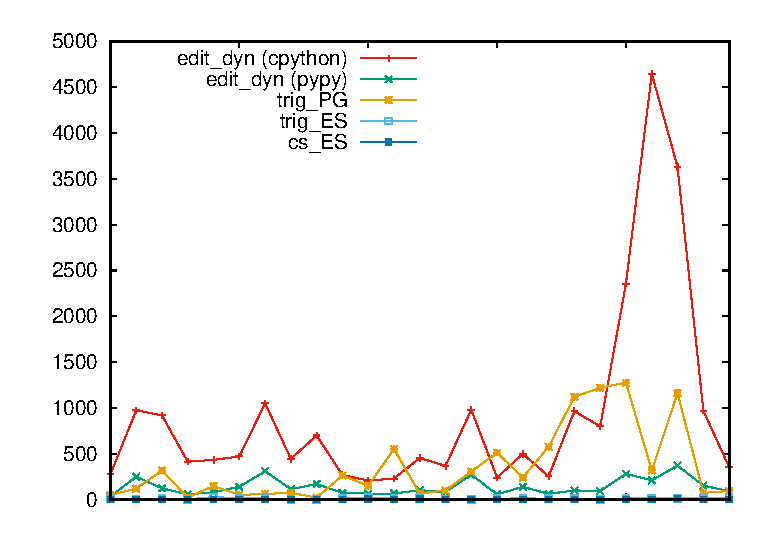
\includegraphics{figures/timings.eps}
\caption{Rychlost vykonání dotazu}
\label{fig:timings}
\end{figure}
\end{minipage}
\begin{minipage}{.45\textwidth}\vspace{0pt}
\begin{figure}[H]
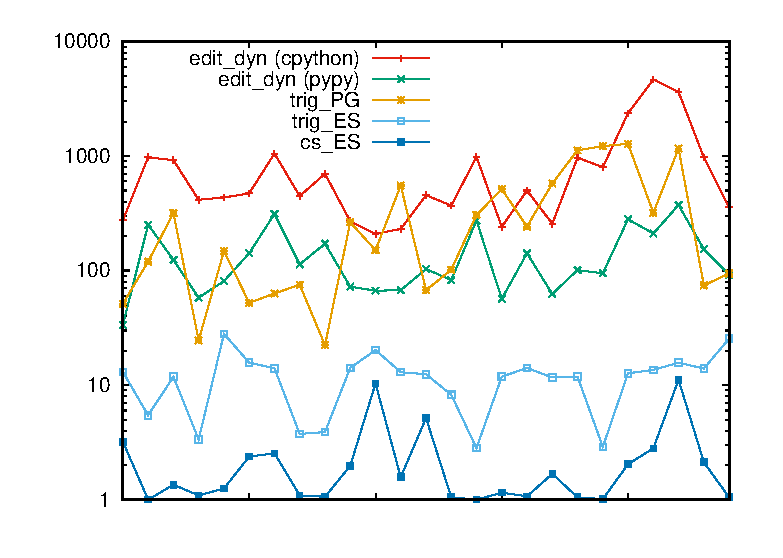
\includegraphics{figures/timings_log.eps}
\caption{Rychlost vykonání dotazu log}
\label{fig:timings_log}
\end{figure}
\end{minipage}
\mbox{}

\noindent\makebox[\textwidth][c]{%
    \begin{minipage}[H]{.5\textwidth}\vspace{0pt}
    \begin{figure}[H]
    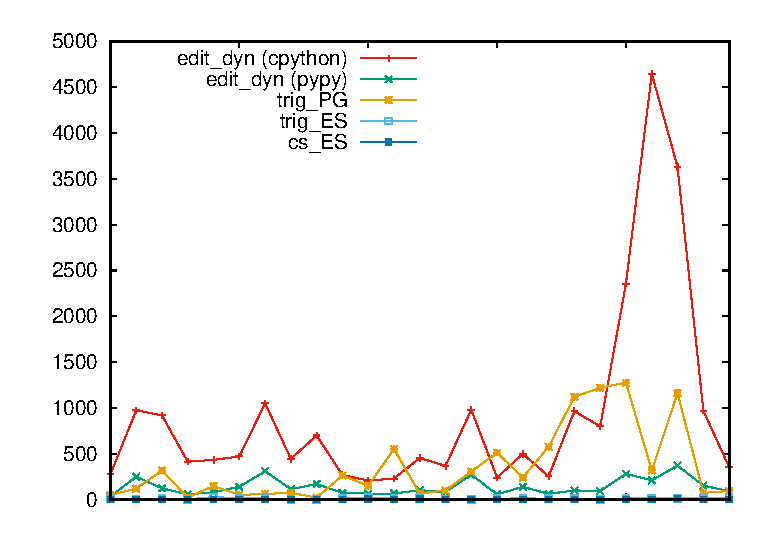
\includegraphics[width=\textwidth]{figures/timings.eps}
    \captionsetup{justification=centering}
    \caption{Rychlost dotazu \bftt{[ms]}}
    \label{fig:timings}
    \end{figure}
    \end{minipage}
    \begin{minipage}[H]{.5\textwidth}\vspace{0pt}
    \begin{figure}[H]
    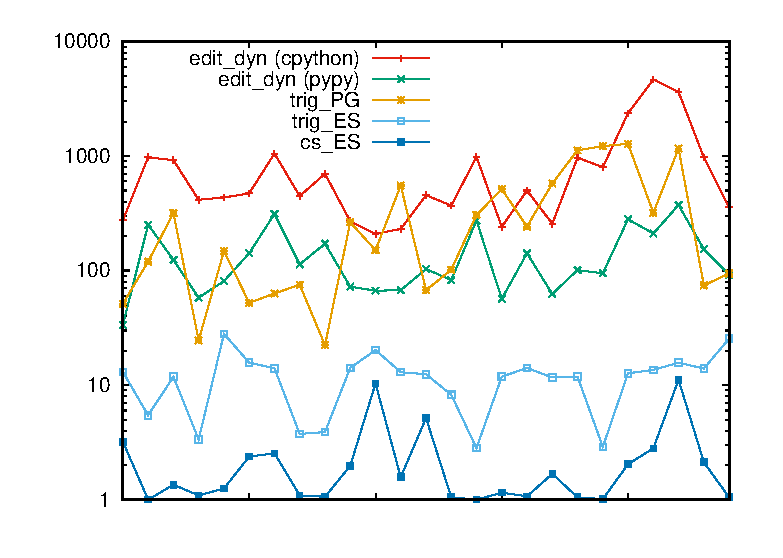
\includegraphics[width=\textwidth]{figures/timings_log.eps}
    \captionsetup{justification=centering}
    \caption{Rychlost dotazu \bftt{log[y] [ms]}}
    \label{fig:timings_log}
    \end{figure}
    \end{minipage}}
\mbox{}\\

Pro porovnání výkonu bylo náhodně zvoleno 24 dotazů pro vyhledání v databázi
\bftt{csfd\_filmy}.  . Obrázky \ref{fig:timings} a \ref{fig:timings_log}
porovnávají rychlost běhu dotazu mezi systémy \bftt{edit\_dyn} interpretovaného
v CPythonu, \bftt{edit\_dyn} interpretovaného v PyPy a dvou konfigurací pro
ElasticSearch \bftt{trig\_ES} a \bftt{cs\_ES}.  Časy jsou průměrem 100 běhů
dotazu pro každý ze systémů.

Podle očekávání je implementace \bftt{edit\_dyn} výkonově nejslabší kvůli
dynamicky typovanému Pythonu. Znatelný je rozdíl mezi jednotlivými interpretery
Pythonu. Zejména pro korelované dotazy \bftt{the of}, \bftt{the they} a
\bftt{the than then they thel them thun}, jimž odpovídá v
obr.~\ref{fig:timings_log} špička dosahující až 4000ms. Tyto dotazy byly
záměrně zkonstruovány z nefrekventovanějších slov \bftt{the} a \bftt{of}, aby
ukázaly na nejhorší možný případ. Oproti CPythonu dokáže PyPy rozpoznat
opakující se kód průchodu invertovanými seznamy a efektivně ho vykonat, jak je
patrné z relativního rozdílu těchto dotazů oproti ostatním.

\bftt{trig\_ES} je podle očekávání pomalejší než základní \bftt{cs\_ES}, ale do
takové míry, kdy to pro malou datovou kolekci nevadí.


\noindent\makebox[\textwidth][c]{%
    \begin{minipage}[H]{.5\textwidth}\vspace{0pt}
    \begin{figure}[H]
    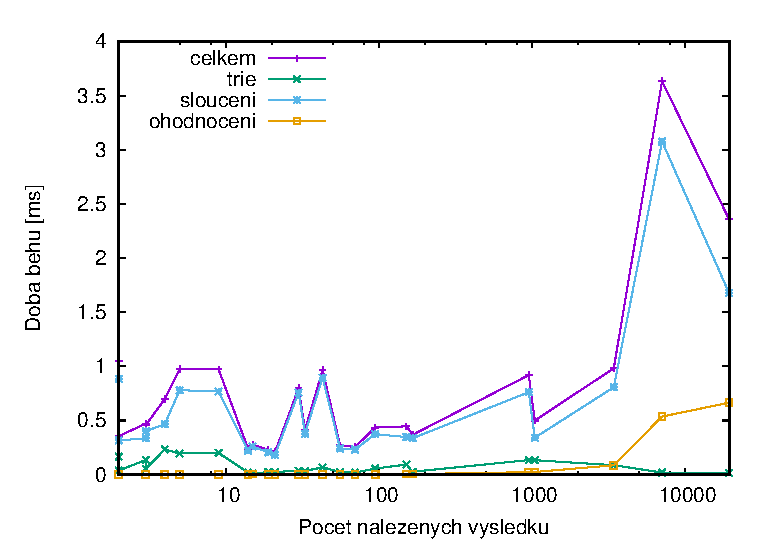
\includegraphics[width=\textwidth]{figures/timings_py_sorted.eps}
    \captionsetup{justification=centering}
    \caption{Rychlost fází \bftt{edit\_dyn} pro CPython \bftt{log[x]}}
    \label{fig:timings_py_sorted}
    \end{figure}
    \end{minipage}
    \begin{minipage}[H]{.5\textwidth}\vspace{0pt}
    \begin{figure}[H]
    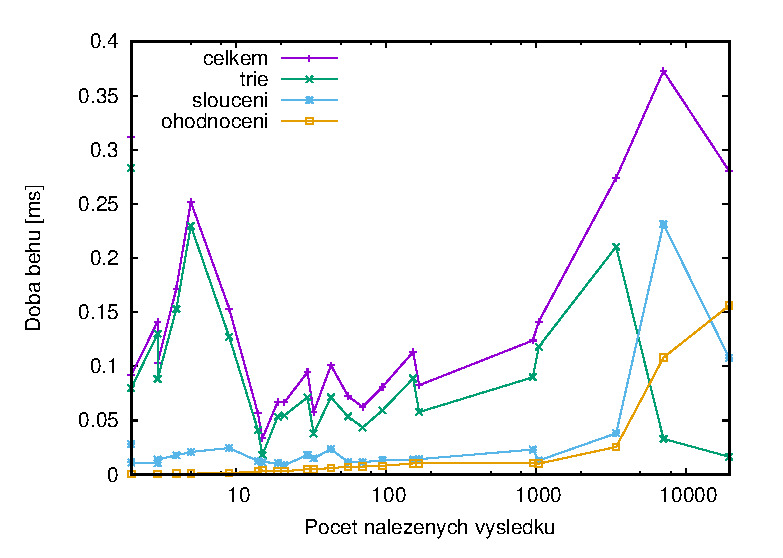
\includegraphics[width=\textwidth]{figures/timings_pypy_sorted.eps}
    \captionsetup{justification=centering}
    \caption{Rychlost fází \bftt{edit\_dyn} pro PyPy \bftt{log[x]}}
    \label{fig:timings_pypy_sorted}
    \end{figure}
    \end{minipage}}

\noindent\makebox[\textwidth][c]{%
    \begin{minipage}[H]{.5\textwidth}\vspace{0pt}
    \begin{figure}[H]
    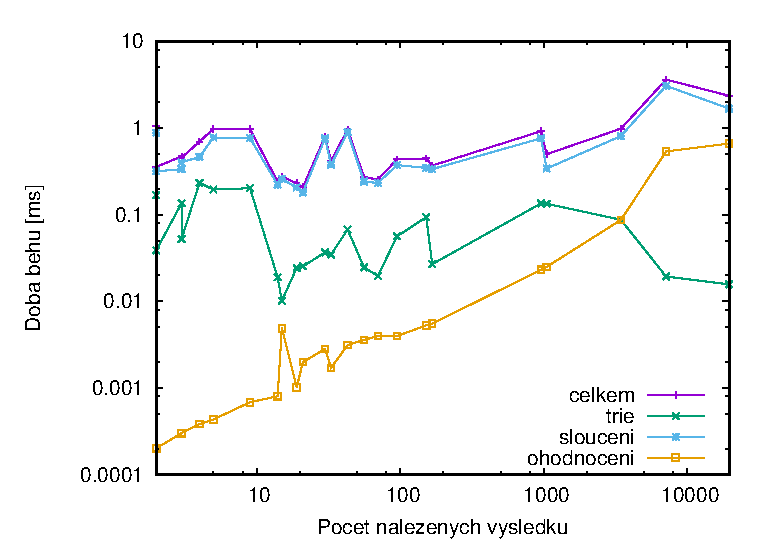
\includegraphics[width=\textwidth]{figures/timings_py_sorted_log.eps}
    \captionsetup{justification=centering}
    \caption{Rychlost fází \bftt{edit\_dyn} pro CPython \bftt{log[x,y]}}
    \label{fig:timings_py_sorted_log}
    \end{figure}
    \end{minipage}
    \begin{minipage}[H]{.5\textwidth}\vspace{0pt}
    \begin{figure}[H]
    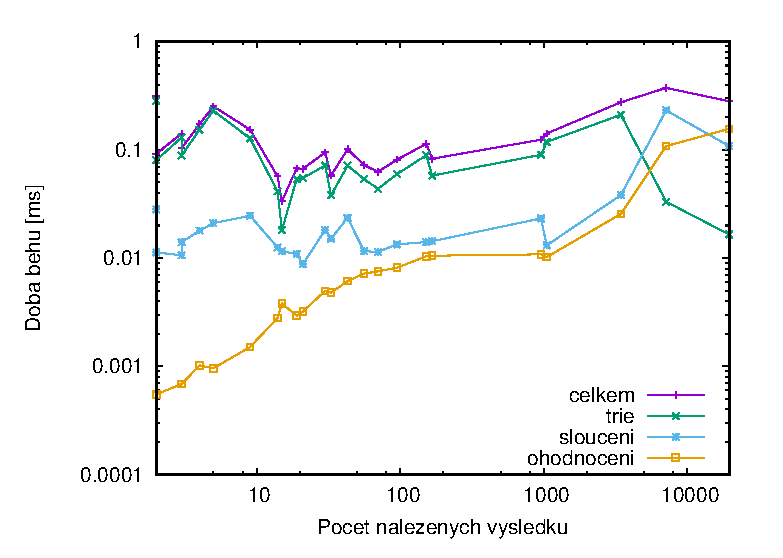
\includegraphics[width=\textwidth]{figures/timings_pypy_sorted_log.eps}
    \captionsetup{justification=centering}
    \caption{Rychlost fází \bftt{edit\_dyn} pro PyPy \bftt{log[x,y]}}
    \label{fig:timings_pypy_sorted_log}
    \end{figure}
    \end{minipage}}
\mbox{}\\

Poměr všech tří fází vykonání dotazu (1. vyhledání podobných slov ve slovníku
\bftt{trie}, 2. sloučení všech odpovídajících invertovaných seznamů
\bftt{slouceni}, 3. ohodnocení nalezených dokumentů \bftt{ohodnoceni}) na
obrázcích \ref{fig:timings_py_sorted}, \ref{fig:timings_pypy_sorted},
\ref{fig:timings_py_sorted_log} a~\ref{fig:timings_pypy_sorted_log} je odlišný
pro různé dotazy. \bftt{ohodnoceni} je přímo závislé na počtu nalezených
výsledků, protože se pro každý z nich aplikuje stejná ohodnocující funkce a
následné seřazení.

Ostatní fáze nejsou na počtu výsledku závislé. \bftt{slouceni} není tolik
závislé díky předsloučeným invertovaným seznamům hybridního uspořádání. Zvýšení
náročnosti je možné pozorovat pro dotazy s frekventovanými slovy \bftt{the} a
\bftt{of}, protože jejich invertované seznamy a disjunkce seznamů s podobnými
slovy jsou delší než u průměrného dotazu. Fáze vyhledání všech slov -
\bftt{trie} - se odvíjí pouze od charakteristiky dat. Tedy pokud existuje více
podobných slov, pak je vykonání delší. Přesto nedosahuje velikých výkyvů.

Za zmínku stojí změna v pořadí fází \bftt{trie} a \bftt{slouceni} mezi
interpretery CPython a PyPy. PyPy si lehce poradí se sloučením invertovaných
seznamů a dominující fází se stane ne tak snadno predikovatelné prohledání ve
slovníku.


%\subsubsection{Porovnání implementací disjunkce}
%\noindent\makebox[\textwidth][c]{%
%    \begin{minipage}[H]{.5\textwidth}\vspace{0pt}
%    \begin{figure}[H]
%    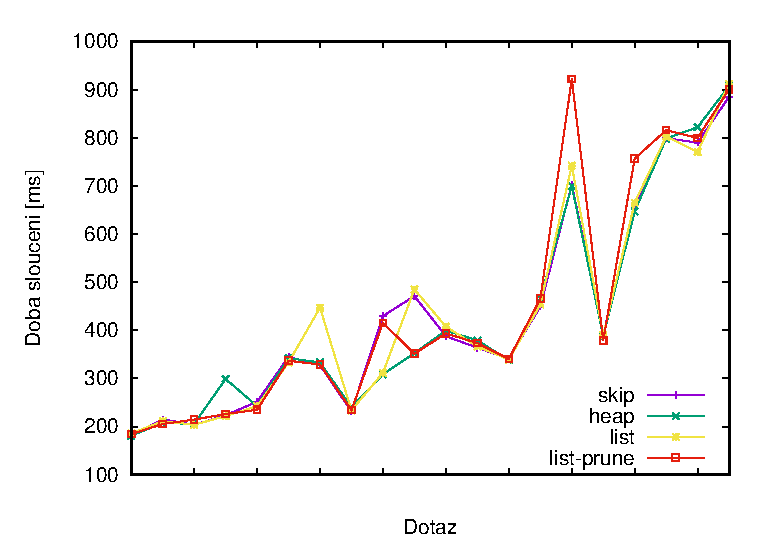
\includegraphics[width=\textwidth]{figures/timings_union_cpython.eps}
%    \captionsetup{justification=centering}
%    \caption{Rychlost sloučení pro CPython}
%    \label{fig:timings_union_cpython}
%    \end{figure}
%    \end{minipage}
%    \begin{minipage}[H]{.5\textwidth}\vspace{0pt}
%    \begin{figure}[H]
%    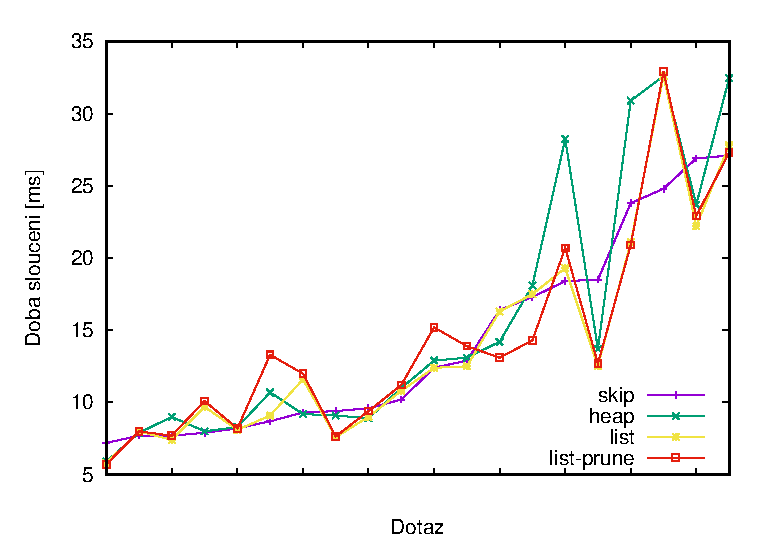
\includegraphics[width=\textwidth]{figures/timings_union_pypy3.eps}
%    \captionsetup{justification=centering}
%    \caption{Rychlost sloučení pro PyPy}
%    \label{fig:timings_union_pypy}
%    \end{figure}
%    \end{minipage}}
%\mbox{}\\

Pro srovnání byly naimplementovány čtyři různé druhy vykonání disjunkce
invertovaných seznamů, které následně figurují v konjunktivním sloučení.

\bftt{heap} je klasické sloučení za pomocí binární haldy, které se hodí, pokud
je invertovaných seznamů mnoho. Kvůli hybridizaci invertovaných seznamů jich
tolik není, a proto by měly být minimálně stejně účinné implementace, kde
prioritní frontu tvoří pouhý lineární seznam - \bftt{list}. \bftt{list-prune}
je obdobou, pouze s tím, že z prioritní fronty odstraní invertované seznamy,
které se dostaly do konce. \bftt{skip} je experimentální implementace
optimalizující přeskakování v invertovaných seznamech oproti postupnému
posunování po jednom dokumentu.

% V obr.~\ref{fig:timings_union_cpython}~a~\ref{fig:timings_union_pypy} jsou
% porovnání těchto implementací pro CPython a Pypy na dvaceti náhodně
% vygenerovaných dotazech. Obrázky jsou seřazeny vzestupně podle implementace
% \bftt{skip}. Žádná ze čtyř implementací nemá dle výsledků v obecném případě
% zásadní vliv na dobu vykonání dotazu. Každá je v některém případě víceméně tou
% nejméně vhodnou a naopak.


\noindent\makebox[\textwidth][c]{%
    \begin{minipage}[H]{.5\textwidth}\vspace{0pt}
    \begin{figure}[H]
    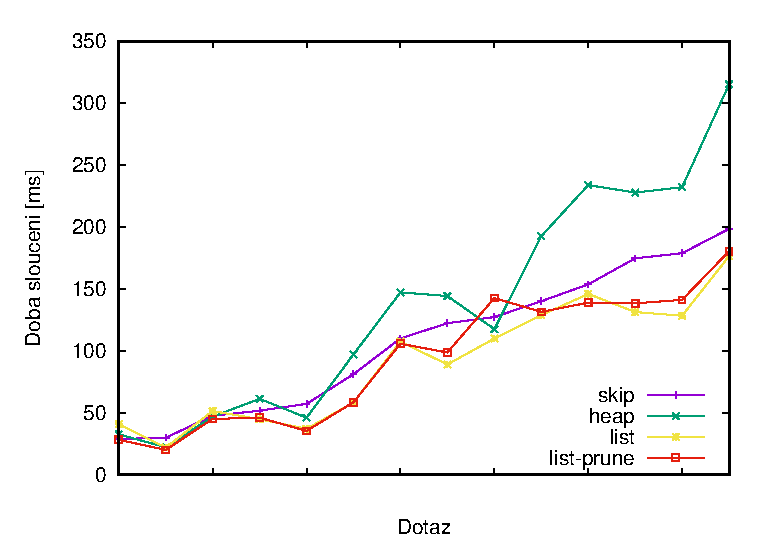
\includegraphics[width=\textwidth]{figures/prefix_union_dense.eps}
    \captionsetup{justification=centering}
    \caption{Rychlost sloučení pro PyPy - prefixový dotaz \bftt{[x* y*]}}
    \label{fig:timings_prefix_union_x_y}
    \end{figure}
    \end{minipage}
    \begin{minipage}[H]{.5\textwidth}\vspace{0pt}
    \begin{figure}[H]
    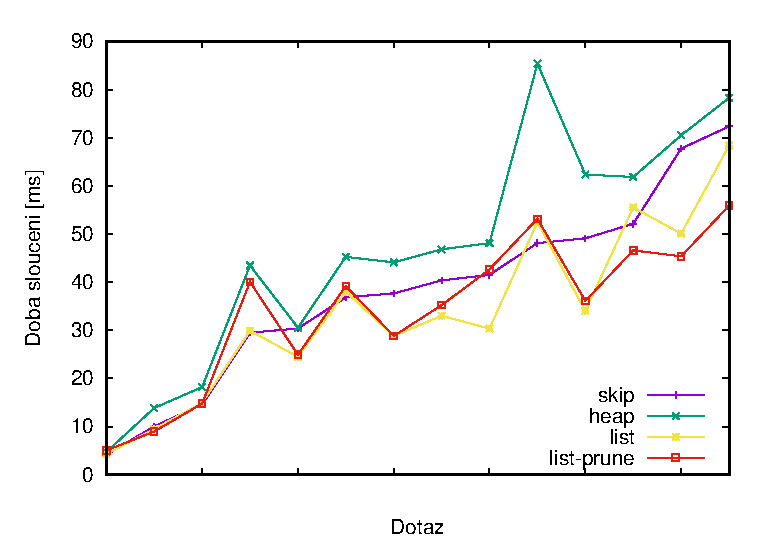
\includegraphics[width=\textwidth]{figures/prefix_union_sparse.eps}
    \captionsetup{justification=centering}
    \caption{Rychlost sloučení pro PyPy - prefixový dotaz \bftt{[x* yy*]}}
    \label{fig:timings_prefix_union_x_yy}
    \end{figure}
    \end{minipage}}

\noindent\makebox[\textwidth][c]{%
    \begin{minipage}[H]{.5\textwidth}\vspace{0pt}
    \begin{figure}[H]
    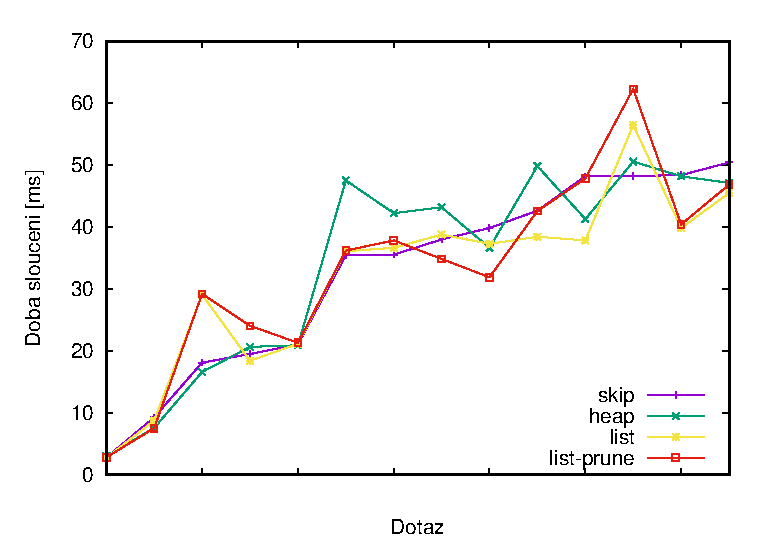
\includegraphics[width=\textwidth]{figures/prefix_union_sparse2.eps}
    \captionsetup{justification=centering}
    \caption{Rychlost sloučení pro PyPy - prefixový dotaz \bftt{[x* yyyy*]}}
    \label{fig:timings_prefix_union_x_yyyy}
    \end{figure}
    \end{minipage}
    \begin{minipage}[H]{.5\textwidth}\vspace{0pt}
    \begin{figure}[H]
    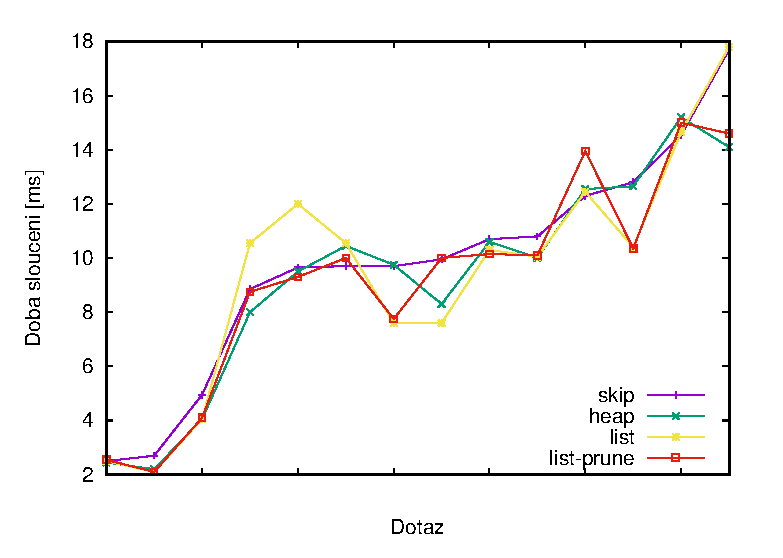
\includegraphics[width=\textwidth]{figures/prefix_union_sparse3.eps}
    \captionsetup{justification=centering}
    \caption{Rychlost sloučení pro PyPy - prefixový dotaz \bftt{[xxxx* yyyy*]}}
    \label{fig:timings_prefix_union_xxxx_yyyy}
    \end{figure}
    \end{minipage}}
\mbox{}\\

Obrázky~\ref{fig:timings_prefix_union_x_y},~\ref{fig:timings_prefix_union_x_yy},~\ref{fig:timings_prefix_union_x_yyyy}
a \ref{fig:timings_prefix_union_xxxx_yyyy} demonstrují rychlost vykonání
náhodných prefixových dotazů. U prefixových dotazů najde slovník velké množství
odpovídajících slov ke každému dotazovanému slovu. Dotazu typu \bftt{x* yyyy*}
v obr.~\ref{fig:timings_prefix_union_x_yyyy} znamená dotaz o dvou prefixech.
\bftt{x} a \bftt{yyyy} znázorňují šablony vygenerovaných slov. Tedy náhodně
vygenerovaný dotaz může vypadat například jako \bftt{s* bene*} nebo \bftt{m*
tolu*}. U dotazu \bftt{x* y*} očekáváme silný vliv disjunkce na dobu vykonání
sloučení, protože prefix pouze o jednom znaku odpovídá velkému množství slov. V
kontrastu dotaz typu \bftt{xxxx* yyyy*}  bude obsahovat menší množství seznamů
v disjunkci. Dotazy typu \bftt{x* yy*} a \bftt{x* yyyy*} slouží k porovnání
schopnost implementací přeskakovat dokumenty v kombinaci řídké (\bftt{yyyy*}) a
husté (\bftt{x*}) disjunkce. Podle očekávání by měla dominovat implementace
\bftt{skip}, ale není tomu tak. Nejvhodnější implementací se ukázala
jednoduchost obyčejného seznamu v případech \bftt{list} a \bftt{list-prune}.

\mbox{}\\
\noindent\makebox[\textwidth][c]{%
    \begin{minipage}[H]{.5\textwidth}\vspace{0pt}
    \begin{figure}[H]
    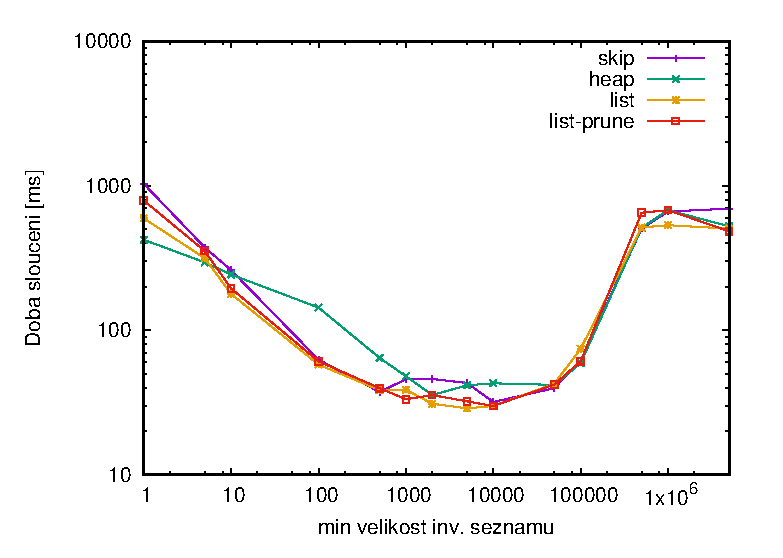
\includegraphics[width=\textwidth]{figures/hybrid_union_s_tebou.eps}
    \captionsetup{justification=centering}
    \caption{Rychlost sloučení pro PyPy - prefixový dotaz \bftt{[s* tebou*]}}
    \label{fig:hybrid_union_s_tebou}
    \end{figure}
    \end{minipage}
    \begin{minipage}[H]{.5\textwidth}\vspace{0pt}
    \begin{figure}[H]
    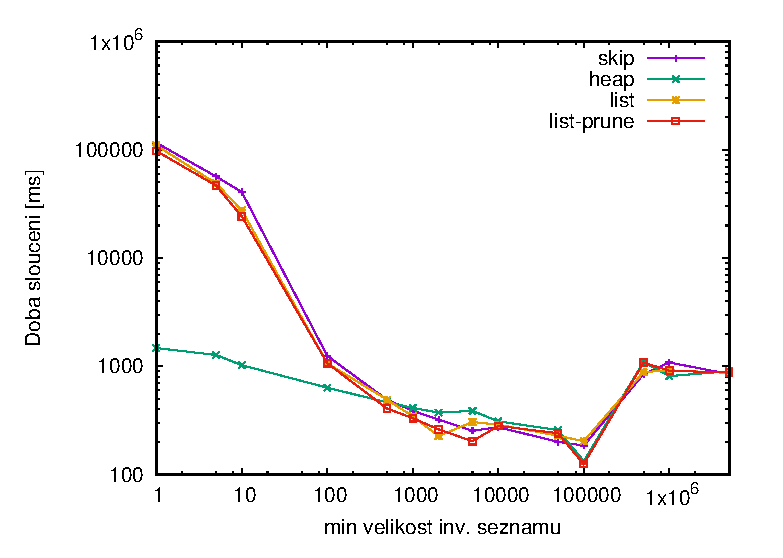
\includegraphics[width=\textwidth]{figures/hybrid_union_s_t.eps}
    \captionsetup{justification=centering}
    \caption{Rychlost sloučení pro PyPy - prefixový dotaz \bftt{[s* t*]}}
    \label{fig:hybrid_union_s_t}
    \end{figure}
    \end{minipage}}
\mbox{}\\

Klíčovým srovnáním této práce je závislost rychlosti sloučení invertovaných
seznamů na velikosti seskupení invertovaných seznamů (TODO ref algorithmus).
Pro porovnání byla datová sada \bftt{csfd\_filmy} zaindexována pro více
parametrů seskupení a pro každý takový index byla změřena doba sloučení pro
prefixové dotazy \bftt{s* tebou*} (reprezentující typ dotazu \bftt{x* yyyyy*},
obr.~\ref{fig:hybrid_union_s_tebou}), a dotaz \bftt{s* t*} (reprezentující
\bftt{x* y*}, obr.~\ref{fig:hybrid_union_s_t}). Parametrem seskupení se rozumí
minimální velikost seskupeného invertovaného seznamu. Tedy klasický invertovaný
index bez hybridního sloučení odpovídá hodnotě 1. Naopak úplný dopředný index
má maximálně možně dlouhý invertovaný seznam o velikosti počtu všech slov v
datové sadě (v tomto případě je v databázi \bftt{csfd\_filmy} 1\,958\,147
výskytů slov). Lidsky řečeno, čím více vlevo v
obr.~\ref{fig:hybrid_union_s_tebou}~a~\ref{fig:hybrid_union_s_t}, tím je index
\uv{více invertovaný}. Naopak, čím více vpravo, tím index více připomíná
původní datovou kolekci. Křivky jsou v hodnotách 500\,000 a výše téměř totožné,
protože pro oba dotazy už jsou jejich invertované seznamy předsloučené a při
průchodu už dochází pouze k jejich filtrování.

Zajímavým pozorováním je absolutní nevhodnost klasického invertovaného seznamu
pro krátké prefixové dotazy. V takovém případě dochází k masivnímu sloučení
mnoha krátkých invertovaných seznamů. Podle očekávání zde uplatňuje
implementace \bftt{heap}, jejíž složitost nalezení následujícího dokumentu je
$\log n$ oproti ostatním, které procházejí disjunktivní seznam lineárně.



\subsection{Hledání ve slovníku}
\noindent\makebox[\textwidth][c]{%
    \begin{minipage}[H]{.5\textwidth}\vspace{0pt}
    \begin{figure}[H]
    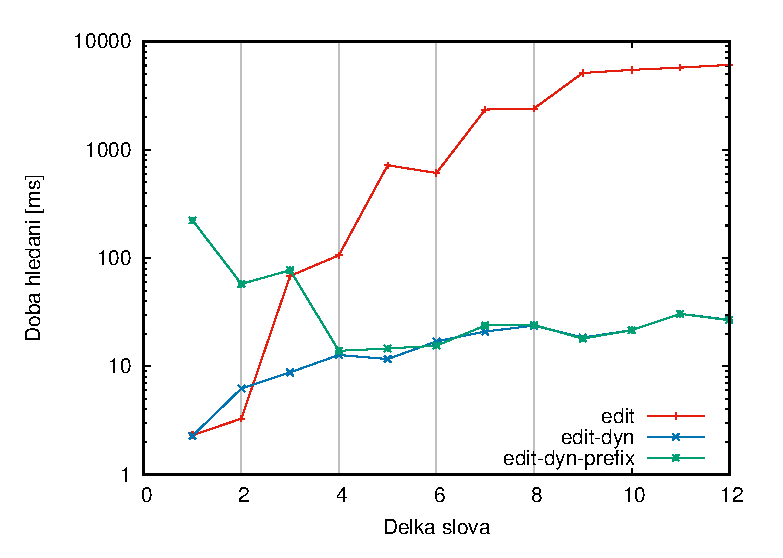
\includegraphics[width=\textwidth]{figures/trie_edit_cpython.eps}
    \captionsetup{justification=centering}
    \caption{Rychlost slovníku (v~CPythonu)~\bftt{log[y]}}
    \label{fig:trie_edit_cpython}
    \end{figure}
    \end{minipage}
    \begin{minipage}[H]{.5\textwidth}\vspace{0pt}
    \begin{figure}[H]
    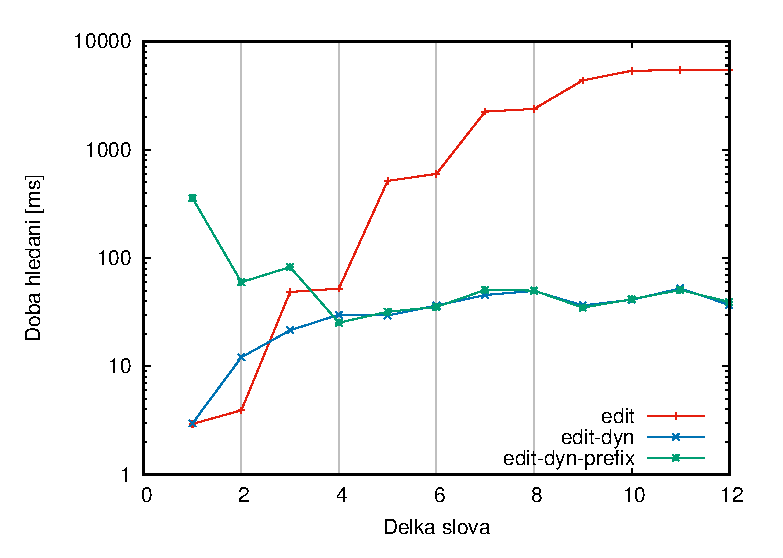
\includegraphics[width=\textwidth]{figures/trie_edit_pypy3.eps}
    \captionsetup{justification=centering}
    \caption{Rychlost slovníku (v~PyPy)~\bftt{log[y]}}
    \label{fig:trie_edit_pypy}
    \end{figure}
    \end{minipage}}
\mbox{}\\

Jedním z důvodů, proč je dynamicky prořezávaná editovací vzdálenost výhodná je
její časová náročnost, protože se, narozdíl od běžné, vyhýbá drahému průchodu
podstromy u počátečních znaků.
Obr.~\ref{fig:trie_edit_pypy}~a~\ref{fig:trie_edit_cpython} znázorňují
závislost tří variant editovací vzdálenosti při průchodu prefixovým stromem a
nalezením všech podobných slov. \bftt{edit} je klasická Levenshteinova
vzdálenost, \bftt{edit-dyn} je dynamicky prořezávaná varianta a
\bftt{edit-dyn-prefix} je předchozí varianta, která vyhledává prefixově.
Vertikální čáry znázorňují zvýšení práhu editovací vzdálenosti. Ta začíná na
nule - tedy nejkratší slova se hledají přesně, a na délkách 2, 4, 6, 8 se
zvedne o jeden bod (slova o délce 3 se hledají s práhem 1, o délce 5 s práhem
2, ...). Dlouhé vykonání u krátkých slov u \bftt{edit-dyn-prefix} je způsobeno
vyčerpávajícím průchodem všemi slovy, které odpovídají prefixu. Dynamické
prořezávání je výhodné, protože umožňuje bez větší ztráty vyšší toleranci
editační vzdálenosti s rostoucí délkou slova.

Narozdíl od sloučení invertovaných seznamů není u vyhledání ve slovníku patrná
výhoda PyPy oproti CPythonu. Dokonce je u \bftt{edit-dyn} a
\bftt{edit-dyn-prefix} CPython výkonnější, což naznačuje, že JIT kompilace PyPy
v tomto případě nepřinesla žádný lepší výkon. Implementace slovníku v jazyce s
překladem do nativního kódu by měla být znatelně rychlejší.



\subsection{Velikost indexu}
ElasticSearch nabízí bod API se statistikami, které nám řeknou i velikost místa
zabraného indexem. Alternativně lze velikost indexu zjistit sečtením velikostí
všech uložených souborů. Obě metody vracejí zhruba stejné výsledky ($\pm 4\%$).

Indexy pro vyhledávače \bftt{edit} a \bftt{edit\_dyn} jsou totožné. Liší se
pouze formou hledání podobných slov ve slovníku.

\begin{Verbatim}
# Součet souborů na disku
du -shc //elasticsearch/nodes/*/indices/<index>/*/index/*

# Využití statistik skrz API
http '<uri>/<index>/_stats' | jq .indices.<index>.primaries.store.size_in_bytes
\end{Verbatim}

\begin{tt}
\begin{table}[H]
\centering
\begin{tabulary}{\textwidth}{LLRR}
\textbf{databáze} & \textbf{implementace} & \textbf{velikost indexu} \\
\hline
\multirow{3}{*}{\texttt{csfd\_filmy}} & trigram\_ES & 86\,MB \\
                                      & cs\_ES      & 37\,MB \\
                                      & edit        & 42\,MB \\
\hline
\multirow{3}{*}{\texttt{csfd\_tvůrci}} & trigram\_ES & 31\,MB \\
                                       & cs\_ES & 14\,MB \\
                                       & edit & 15\,MB \\
\hline
\multirow{3}{*}{\texttt{cswiki\_titulky}} & trigram\_ES & 135\,MB \\
                                          & cs\_ES & 63\,MB \\
                                          & edit & 63\,MB \\
\hline
\end{tabulary}
\caption{Velikosti indexů}
\label{tab:index_size}
\end{table}
\end{tt}

\chapter{Další postup a otevřené problémy}
\section{Integrace do existujících systémů}
\section{Statické a dynamické indexy}
% static: no locks and latches, compact data structures, cache efficient
% 2 level data structure + bulk updates
% columnar storage
% document or term based
% share nothing
\section{Příliš krátký vstupní řetězec}
\section{Plánování dotazů}
\section{Ukládání inkrementálních mezivýsledků}
\section{Zvýrazňovač pro editační vzdálenost}
\section{Škálovatelnost}
V této práci je mým cílem poukázat, že pro malá objemy dat je vhodné použít
adekvátní techniky pro zvýšení relevance vyhledávání za cenu zvýšené výpočetní
náročnosti. Tím, že jsou počítače stále výkonnější a datové sady se snadno
vejdou do dostupné paměti RAM, neměl by být při efektivní implementaci a
běžných dotazech s výkonem problém. Pokud jsou požadavkem větší objemy dat,
protože například firma roste s přibývajícím počtem zákazníků, pak by dnes
neměl být problém dokoupit si více paměti, která je každým rokem stále levnější.

I kdyby nepřipadalo v úvahu vertikální škálování přidáváním více RAM, existuje
možnost horizontálního škálování na více počítačů a vytvoření distribuovaného
systému. Invertované indexy jsou velmi snadno paralelizovatelné problémy
% TODO term or document distributed. cite something

Ten by ostatně byl nezbytný, pokud by požadavkem byla vysoká
dostupnost dat. Stejná data by byla replikována na více strojů a v případě
selhání jednoho by se instantně použila redundance více strojů.



\subsubsection{Indexování}
Implementace je zaměřená především na ty části, které jsou klíčové pro
demonstraci návrhu. Indexovací fáze používá jednoduchý \bftt{sort based}
algoritmus a nevyužívá techniky více souborů. Do budoucna by bylo užitečné
zjistit, jaké jsou nejvhodnější indexovací metody pro hybridní index oproti
klasickému invertovanému indexu.

\subsubsection{Porovnání výkonu}
Algoritmy pro slučování invertovaných seznamů jsou obzvlášť citlivé na správnou
implementaci a především na zvolený programovací jazyk. Zatímco Python je
ideální prototypovací jazyk, je asi tím nejhorším, v čem by měl být produkční
vyhledávací systém vytvořen. To se sice časem může změnit díky výkonově
orientovanému interpreteru PyPy. Přesto by měla být pro adekvátní porovnání
implementace provedena v jazyce s podporou překladu do nativního strojového
kódu.

Se zpomalujícím Mooreovým zákonem se objevují různé formy paralelismu, které by
měly sloužit jako náhrada za klesající tempo růstu. Pro pečlivě optimalizovaný
kód, které databázové a vyhledávací systémy často využívají, se častěji a
častěji využívají bitově-paralelní instrukce moderních procesorů. I z tohoto
důvodu by měl být zvolen takový jazyk, ve kterém není velkou překážkou tyto
moderní schopnosti procesorů využívat. (cite completesearch C++).


\chapter{Závěr}
Záměrem této práce je poukázat na alternativní techniky v oblasti vyhledávání a
demonstrovat možný vyhledávací systém, který je implementuje. Tento systém by
měl být vhodnější pro potřeby jednotlivců i firem, které vyžadují od
vyhledávacího systému robustnost proti malým změnám v dotazu. Uplatnění by měl
nalézt v menších datových sadách, než na které je dnes kladen důraz, protože
díky omezené velikosti dat je možné přebytečný výpočetní výkon použít k těmto
náročnějším technikám.

Navržený vyhledávací systém byl implementován jako prototyp obsahující popsané
techniky a porovnán s několika dalšími vyhledávači, které byly vytvořeny jako
různé konfigurace v některých populárních open source vyhledávacích systémech
tak, aby odpovídaly popsaným požadavkům.

Implementovaný prototyp byl vytvořen tak, aby byl schopný v první řadě
demonstraci popsaných technik a byl dostatečně flexibilní pro potřeby
experimentování. Výkonově není reprezentativní kvůli implementaci v zvoleném
dynamicky typovaném programovacím jazyce Python, ale byla použita stejná
architektura, kterou by bylo možné pouze přepsat do výkonnějšího jazyka. Bylo
proto provedeno relativní porovnání výkonu mezi určitými typy dotazů s vyšší
mírou tolerance pro běh dotazu, které ukázalo že pro běžný dotaz by vyhledávač
splňoval kritéria pro vyhledávání v reálném čase. 

Analýza nejhorších případů ukázala na typ dotazů, které by mohly být zneužity
proti vyhledávači. Pro tento případ byl nastíněn způsob, jak ho řešit, ač by
zkomplikoval původně jednoduchou architekturu.

V porovnání s alternativami založených na ngramové podobnosti není navržený
systém robustní v případech oddělených slov nebo naopak kompozitních slov.
Možným dalším rozšířením by byla kombinace navržené architektury s ngramy.

\section*{Odkazy}
\url{http://www.dcs.gla.ac.uk/~craigm/publications/lacour08efficiency.pdf}

\newpage
\section*{Reference}
\bibliographystyle{csplainnat}
\bibliography{ref}

\appendix
\chapter{Konfigurace porovnaných systémů v ElasticSearch}\label{appendix:search_config}
\section{ElasticSearch}
\subsection{trigram\_ES}
\subsubsection{Analyzér}
Pro ngramové zaindexování lze použít buď ngramový tokenizér
\bftt{my\_ngram\_tokenizer}, nebo ngramový filtr \bftt{my\_ngram\_filter}.
Ngramový tokenizér podporuje zvýrazňování, které se mi s ngramovým filtrem
nepovedlo nastavit ani po vyčerpávajícím hledání. Ve výpisu konfigurace jsou
uvedeny oba způsoby nastavení. \bftt{my\_short\_words\_filter} vybírá slova
zahozená tokenizérem \bftt{my\_ngram\_tokenizer}, proto je v něm nastavena
maximální délka menší než délka trigramu - 2.

\begin{Verbatim}[commandchars=\\\{\}]
\PY{p}{\PYZob{}}
  \PY{n+nt}{\PYZdq{}settings\PYZdq{}}\PY{p}{:} \PY{p}{\PYZob{}}
    \PY{n+nt}{\PYZdq{}analysis\PYZdq{}}\PY{p}{:} \PY{p}{\PYZob{}}
      \PY{n+nt}{\PYZdq{}tokenizer\PYZdq{}}\PY{p}{:} \PY{p}{\PYZob{}}
        \PY{n+nt}{\PYZdq{}my\PYZus{}ngram\PYZus{}tokenizer\PYZdq{}}\PY{p}{:} \PY{p}{\PYZob{}}
          \PY{n+nt}{\PYZdq{}type\PYZdq{}}\PY{p}{:} \PY{l+s+s2}{\PYZdq{}nGram\PYZdq{}}\PY{p}{,}
          \PY{n+nt}{\PYZdq{}min\PYZus{}gram\PYZdq{}}\PY{p}{:} \PY{l+m+mi}{3}\PY{p}{,}
          \PY{n+nt}{\PYZdq{}max\PYZus{}gram\PYZdq{}}\PY{p}{:} \PY{l+m+mi}{3}\PY{p}{,}
          \PY{n+nt}{\PYZdq{}token\PYZus{}chars\PYZdq{}}\PY{p}{:} \PY{p}{[}\PY{l+s+s2}{\PYZdq{}letter\PYZdq{}}\PY{p}{,} \PY{l+s+s2}{\PYZdq{}digit\PYZdq{}}\PY{p}{]}
        \PY{p}{\PYZcb{}}
      \PY{p}{\PYZcb{}}\PY{p}{,}
      \PY{n+nt}{\PYZdq{}filter\PYZdq{}}\PY{p}{:} \PY{p}{\PYZob{}}
        \PY{n+nt}{\PYZdq{}my\PYZus{}ngram\PYZus{}filter\PYZdq{}}\PY{p}{:} \PY{p}{\PYZob{}}
          \PY{n+nt}{\PYZdq{}type\PYZdq{}}\PY{p}{:} \PY{l+s+s2}{\PYZdq{}ngram\PYZdq{}}\PY{p}{,}
          \PY{n+nt}{\PYZdq{}min\PYZus{}gram\PYZdq{}}\PY{p}{:} \PY{l+m+mi}{3}\PY{p}{,}
          \PY{n+nt}{\PYZdq{}max\PYZus{}gram\PYZdq{}}\PY{p}{:} \PY{l+m+mi}{3}
        \PY{p}{\PYZcb{}}\PY{p}{,}
        \PY{n+nt}{\PYZdq{}my\PYZus{}short\PYZus{}words\PYZus{}filter\PYZdq{}}\PY{p}{:} \PY{p}{\PYZob{}}
            \PY{n+nt}{\PYZdq{}type\PYZdq{}}\PY{p}{:} \PY{l+s+s2}{\PYZdq{}length\PYZdq{}}\PY{p}{,}
            \PY{n+nt}{\PYZdq{}max\PYZdq{}}\PY{p}{:} \PY{l+m+mi}{2}
        \PY{p}{\PYZcb{}}
      \PY{p}{\PYZcb{}}\PY{p}{,}
      \PY{n+nt}{\PYZdq{}analyzer\PYZdq{}}\PY{p}{:} \PY{p}{\PYZob{}}
        \PY{n+nt}{\PYZdq{}my\PYZus{}ngrams\PYZdq{}}\PY{p}{:} \PY{p}{\PYZob{}}
          \PY{n+nt}{\PYZdq{}type\PYZdq{}}\PY{p}{:} \PY{l+s+s2}{\PYZdq{}custom\PYZdq{}}\PY{p}{,}
          \PY{n+nt}{\PYZdq{}tokenizer\PYZdq{}}\PY{p}{:} \PY{l+s+s2}{\PYZdq{}my\PYZus{}ngram\PYZus{}tokenizer\PYZdq{}}\PY{p}{,}
          \PY{n+nt}{\PYZdq{}filter\PYZdq{}}\PY{p}{:} \PY{p}{[}
            \PY{l+s+s2}{\PYZdq{}asciifolding\PYZdq{}}\PY{p}{,}
            \PY{l+s+s2}{\PYZdq{}lowercase\PYZdq{}}
          \PY{p}{]}
        \PY{p}{\PYZcb{}}\PY{p}{,}
        \PY{n+nt}{\PYZdq{}my\PYZus{}standard\PYZdq{}}\PY{p}{:} \PY{p}{\PYZob{}}
            \PY{n+nt}{\PYZdq{}type\PYZdq{}}\PY{p}{:} \PY{l+s+s2}{\PYZdq{}custom\PYZdq{}}\PY{p}{,}
            \PY{n+nt}{\PYZdq{}tokenizer\PYZdq{}}\PY{p}{:} \PY{l+s+s2}{\PYZdq{}standard\PYZdq{}}\PY{p}{,}
            \PY{n+nt}{\PYZdq{}filter\PYZdq{}}\PY{p}{:} \PY{p}{[}
                \PY{l+s+s2}{\PYZdq{}asciifolding\PYZdq{}}\PY{p}{,}
                \PY{l+s+s2}{\PYZdq{}lowercase\PYZdq{}}
            \PY{p}{]}
        \PY{p}{\PYZcb{}}\PY{p}{,}
        \PY{n+nt}{\PYZdq{}my\PYZus{}short\PYZus{}words\PYZdq{}}\PY{p}{:} \PY{p}{\PYZob{}}
            \PY{n+nt}{\PYZdq{}type\PYZdq{}}\PY{p}{:} \PY{l+s+s2}{\PYZdq{}custom\PYZdq{}}\PY{p}{,}
            \PY{n+nt}{\PYZdq{}tokenizer\PYZdq{}}\PY{p}{:} \PY{l+s+s2}{\PYZdq{}standard\PYZdq{}}\PY{p}{,}
            \PY{n+nt}{\PYZdq{}filter\PYZdq{}}\PY{p}{:} \PY{p}{[}
                \PY{l+s+s2}{\PYZdq{}asciifolding\PYZdq{}}\PY{p}{,}
                \PY{l+s+s2}{\PYZdq{}lowercase\PYZdq{}}\PY{p}{,}
                \PY{l+s+s2}{\PYZdq{}my\PYZus{}short\PYZus{}words\PYZus{}filter\PYZdq{}}
            \PY{p}{]}
        \PY{p}{\PYZcb{}}\PY{p}{\PYZcb{}}\PY{p}{\PYZcb{}}\PY{p}{\PYZcb{}}\PY{p}{\PYZcb{}}
\end{Verbatim}


\subsubsection{Mapování}
Aby fungoval zvýrazňovač pro ngramové indexy, musí být použit \bftt{Fast
Vector Highlighter}, který funguje, pokud se pro pole nastaví hodnota
\bftt{with\_position\_offsets} u parametru \bftt{term\_vector}. Nicméně
nakonec byl použit externí zvýrazňovač, proto by mohlo být ukládání této
informace vypnuto. Doporučuje se ji použít pro dlouhé texty, což není
případ použitých datových sad v této práci.

\begin{Verbatim}[commandchars=\\\{\}]
\PY{p}{\PYZob{}}
  \PY{n+nt}{\PYZdq{}properties\PYZdq{}}\PY{p}{:} \PY{p}{\PYZob{}}
    \PY{n+nt}{\PYZdq{}title\PYZdq{}}\PY{p}{:} \PY{p}{\PYZob{}}
        \PY{n+nt}{\PYZdq{}type\PYZdq{}}\PY{p}{:} \PY{l+s+s2}{\PYZdq{}multi\PYZus{}field\PYZdq{}}\PY{p}{,}
        \PY{n+nt}{\PYZdq{}fields\PYZdq{}}\PY{p}{:} \PY{p}{\PYZob{}}
            \PY{n+nt}{\PYZdq{}title\PYZdq{}}\PY{p}{:} \PY{p}{\PYZob{}}
                \PY{n+nt}{\PYZdq{}type\PYZdq{}}\PY{p}{:} \PY{l+s+s2}{\PYZdq{}string\PYZdq{}}\PY{p}{,}
                \PY{n+nt}{\PYZdq{}analyzer\PYZdq{}}\PY{p}{:} \PY{l+s+s2}{\PYZdq{}my\PYZus{}standard\PYZdq{}}\PY{p}{,}
                \PY{n+nt}{\PYZdq{}term\PYZus{}vector\PYZdq{}}\PY{p}{:} \PY{l+s+s2}{\PYZdq{}with\PYZus{}positions\PYZus{}offsets\PYZdq{}}
            \PY{p}{\PYZcb{}}\PY{p}{,}
            \PY{n+nt}{\PYZdq{}trigram\PYZdq{}}\PY{p}{:} \PY{p}{\PYZob{}}
                \PY{n+nt}{\PYZdq{}type\PYZdq{}}\PY{p}{:} \PY{l+s+s2}{\PYZdq{}string\PYZdq{}}\PY{p}{,}
                \PY{n+nt}{\PYZdq{}analyzer\PYZdq{}}\PY{p}{:} \PY{l+s+s2}{\PYZdq{}my\PYZus{}ngrams\PYZdq{}}\PY{p}{,}
                \PY{n+nt}{\PYZdq{}term\PYZus{}vector\PYZdq{}}\PY{p}{:} \PY{l+s+s2}{\PYZdq{}with\PYZus{}positions\PYZus{}offsets\PYZdq{}}
            \PY{p}{\PYZcb{}}\PY{p}{,}
            \PY{n+nt}{\PYZdq{}shorts\PYZdq{}}\PY{p}{:} \PY{p}{\PYZob{}}
                \PY{n+nt}{\PYZdq{}type\PYZdq{}}\PY{p}{:} \PY{l+s+s2}{\PYZdq{}string\PYZdq{}}\PY{p}{,}
                \PY{n+nt}{\PYZdq{}analyzer\PYZdq{}}\PY{p}{:} \PY{l+s+s2}{\PYZdq{}my\PYZus{}short\PYZus{}words\PYZdq{}}\PY{p}{,}
                \PY{n+nt}{\PYZdq{}term\PYZus{}vector\PYZdq{}}\PY{p}{:} \PY{l+s+s2}{\PYZdq{}with\PYZus{}positions\PYZus{}offsets\PYZdq{}}
            \PY{p}{\PYZcb{}}\PY{p}{\PYZcb{}}\PY{p}{\PYZcb{}}\PY{p}{\PYZcb{}}\PY{p}{\PYZcb{}}
\end{Verbatim}


\subsubsection{Dotaz pro vyhledávání}
Dotaz je navržen, aby došlo k zásahu, pokud dokument obsahuje alespoň
$70\%$ trigramů dotazu. Vyšší hodnoty začaly rychle ztrácet výsledky a
nižší hodnoty vracely příliš šumu.

Dotaz se snaží shodu najít napříč třemi indexy. \bftt{shorts} jsou
ngramy kratší než $3$, protože je ElasticSearch zahazuje. \bftt{title}
obsahuje všechny tokeny dokumentu (titulku filmu) a \bftt{trigram} je
trigramový index. Manipulace s váhami jednotlivých polí nemá velký vliv
na přesnost výsledku.

Zvýrazňování je nastaveno doporučenou formou pro tento typ dotazu, ale
přesto vynechává překrývající se dotazy (viz TODO). Zvýrazňování je
provedeno externím přiloženým programem \bftt{trihigh.py}.

\begin{Verbatim}[commandchars=\\\{\}]
\PY{p}{\PYZob{}}
    \PY{n+nt}{\PYZdq{}min\PYZus{}score\PYZdq{}}\PY{p}{:} \PY{l+m+mf}{0.1}\PY{p}{,}
    \PY{n+nt}{\PYZdq{}size\PYZdq{}}\PY{p}{:} \PY{l+m+mi}{100}\PY{p}{,}
    \PY{n+nt}{\PYZdq{}query\PYZdq{}}\PY{p}{:} \PY{p}{\PYZob{}}
        \PY{n+nt}{\PYZdq{}multi\PYZus{}match\PYZdq{}}\PY{p}{:} \PY{p}{\PYZob{}}
            \PY{n+nt}{\PYZdq{}query\PYZdq{}}\PY{p}{:} \PY{l+s+s2}{\PYZdq{}QUERY\PYZdq{}}\PY{p}{,}
            \PY{n+nt}{\PYZdq{}minimum\PYZus{}should\PYZus{}match\PYZdq{}}\PY{p}{:} \PY{l+s+s2}{\PYZdq{}70\PYZpc{}\PYZdq{}}\PY{p}{,}
            \PY{n+nt}{\PYZdq{}boost\PYZdq{}}\PY{p}{:} \PY{l+m+mi}{2}\PY{p}{,}
            \PY{n+nt}{\PYZdq{}type\PYZdq{}}\PY{p}{:} \PY{l+s+s2}{\PYZdq{}most\PYZus{}fields\PYZdq{}}\PY{p}{,}
            \PY{n+nt}{\PYZdq{}fields\PYZdq{}}\PY{p}{:} \PY{p}{[}
                \PY{l+s+s2}{\PYZdq{}title.shorts\PYZdq{}}\PY{p}{,}
                \PY{l+s+s2}{\PYZdq{}title.title\PYZca{}3.5\PYZdq{}}\PY{p}{,}
                \PY{l+s+s2}{\PYZdq{}title.trigram\PYZca{}2.5\PYZdq{}}
            \PY{p}{]}
        \PY{p}{\PYZcb{}}
    \PY{p}{\PYZcb{}}\PY{p}{,}
    \PY{n+nt}{\PYZdq{}highlight\PYZdq{}}\PY{p}{:} \PY{p}{\PYZob{}}
        \PY{n+nt}{\PYZdq{}pre\PYZus{}tags\PYZdq{}}\PY{p}{:} \PY{p}{[}\PY{l+s+s2}{\PYZdq{}HLSTART\PYZdq{}}\PY{p}{]}\PY{p}{,}
        \PY{n+nt}{\PYZdq{}post\PYZus{}tags\PYZdq{}}\PY{p}{:} \PY{p}{[}\PY{l+s+s2}{\PYZdq{}HLEND\PYZdq{}}\PY{p}{]}\PY{p}{,}
        \PY{n+nt}{\PYZdq{}type\PYZdq{}}\PY{p}{:} \PY{l+s+s2}{\PYZdq{}fvh\PYZdq{}}\PY{p}{,}
        \PY{n+nt}{\PYZdq{}number\PYZus{}of\PYZus{}fragments\PYZdq{}}\PY{p}{:} \PY{l+m+mi}{0}\PY{p}{,}
        \PY{n+nt}{\PYZdq{}fields\PYZdq{}}\PY{p}{:} \PY{p}{\PYZob{}}
            \PY{n+nt}{\PYZdq{}title\PYZdq{}}\PY{p}{:} \PY{p}{\PYZob{}}
                \PY{n+nt}{\PYZdq{}matched\PYZus{}fields\PYZdq{}}\PY{p}{:} \PY{p}{[}
                    \PY{l+s+s2}{\PYZdq{}title.trigram\PYZdq{}}\PY{p}{,}
                    \PY{l+s+s2}{\PYZdq{}title.title\PYZdq{}}\PY{p}{,}
                    \PY{l+s+s2}{\PYZdq{}title.shorts\PYZdq{}}
                \PY{p}{]}
            \PY{p}{\PYZcb{}}\PY{p}{\PYZcb{}}\PY{p}{\PYZcb{}}\PY{p}{\PYZcb{}}
\end{Verbatim}



\backmatter


\end{document}
